\documentclass[12pt,a4paper,oneside,draft]{scrartcl}
\usepackage{amsmath,amssymb}
\usepackage[unicode,colorlinks]{hyperref}
\usepackage{indentfirst,misccorr,mathtext}
\usepackage[russian]{babel}
\usepackage[utf8]{inputenc}
\usepackage[pdftex]{graphicx}
\usepackage{calc}

\usepackage[margin=2cm]{geometry}

\newcounter{notask}
\setcounter{notask}{1}

%Task without picture
\newcommand{\task}[1]{
  \hrule
  \hbox to \textwidth {%
    \vrule
    \parbox[t]{0.04\textwidth}{\smallskip \hfill \arabic{notask} \hfill }
    \vrule
    \hfil
    \parbox[t]{0.93\textwidth}{\smallskip #1 \smallskip}
    \vrule
  }
  \hrule
  \addtocounter{notask}{1}
  \pagebreak[2]
}

%Task with picture
\newcommand{\taskpic}[2]{
  \hrule
  \hbox to \textwidth {%
    \vrule
    \parbox[t]{0.04\textwidth}{\smallskip \hfill \arabic{notask} \hfill }
    \vrule
    \hfil
    \parbox[t]{0.93\textwidth-4.3cm}{\smallskip #1 \smallskip}
    \vrule
    \hfil
    \parbox[t]{4cm}{\smallskip \begin{center}  #2 \end{center}}
    \vrule
  }
  \hrule 
  \addtocounter{notask}{1}
  \pagebreak[2]
}

\newcommand{\com}[1]{{\Large{\texttt{{\color{red}(#1)}}}}}
\newcommand{\unit}[1]{\text{ #1}}
\newcommand{\eps}{\varepsilon}
\pagestyle{empty}
\graphicspath{{./photos/}{./08/battle/}{./09/battle/}{./09/daily/problems/}{./10/daily/problems/}{./10/battle/final/}{./10/battle/semifinal/}{./11/battle/final/}{./11/battle/semifinal/}}

\begin{document}
\parindent=5mm
\section{Общие сведения.}
\label{sec:general}

Летняя Физическая Школа в 2010 году проходила в шестнадцатый
раз. Школа началась 17 июля, а закончилась 6
августа. Продолжительность Школы составила три недели. 

В работе ЛФШ участвовали 67 школьников. Преподавательская и воспитательская
деятельность осуществлялась силами 18 человек.

\subsection{Участники Летней Физической Школы. }
\label{sec:scholars}

В ЛФШ принимаются школьники, перешедшие в 8, 9, 10 или 11 класс. Приём
осуществляется либо по результатам городской или региональной
олимпиады по физике, либо по результатам собеседования с
руководителями смены.
\smallskip

\textbf{8 класс (школьники, закончившие в 2010 году 6 или 7 класс)}
\begin{enumerate}

\item Иванов Владислав, 7 класс, гимназия 177, обладатель диплома II степени городской олимпиады по физике
\item Гуцол Ксения, 7 класс, школа 175, обладательница диплома III степени городской олимпиады по физике
\item Муретова Мария, 7 класс, ФМЛ 239, обладательница похвального отзыва городской олимпиады по физике
\item Портянкин	Егор, 7 класс
\item Порчук Павел, 7 класс, школа 636
\item Коско	Софья, 7 класс, ФМЛ 239
\item Ходунов Павел, 6 класс, ФМЛ 239, обладатель диплома I степени городской олимпиады по математике
\item Ковзель Николай, 6 класс,	школа <<Унисон>>
\item Йона Андрей, 6 класс
\end{enumerate}

\textbf{9 класс}
\begin{enumerate}
\item Базалий Вячеслав, лицей <<ФТШ>>, обладатель диплома I степени городской олимпиады по физике, учащийся ГЦФО
\item Егоров Антон, лицей <<ФТШ>>, обладатель диплома I степени городской олимпиады по физике, учащийся ГЦФО
\item Крачун Дмитрий, ФМЛ 239, обладатель диплома I степени городской олимпиады по физике
\item Погодаев Илья, гимназия 610, обладатель диплома II степени городской олимпиады по физике
\item Гуревич Александр, лицей <<ФТШ>>, обладатель диплома III степени городской олимпиады по физике, учащийся ГЦФО
\item Минкин Алексей, лицей <<ФТШ>>, обладатель диплома III степени городской олимпиады по физике, учащийся ГЦФО
\item Серов Юрий, лицей <<ФТШ>>, обладатель диплома III степени городской олимпиады по физике, учащийся ГЦФО
\item Грудкин Антон, ФМЛ 239, обладатель диплома III степени городской олимпиады по физике
\item Цейтлин Леонид, ФМЛ 30, обладатель диплома III степени городской олимпиады по физике
\item Горбунова Елизавета, лицей <<ФТШ>>, обладательница похвального отзыва городской олимпиады по физике, учащаяся ГЦФО
\item Недошивин Михаил, ФМЛ 239, обладатель похвального отзыва городской олимпиады по физике
\item Капралов Николай, лицей <<ФТШ>>, учащийся ГЦФО
\item Корешкова Ксения, гимназия 114, учащаяся ГЦФО
\item Ковалёв Григорий, ФМЛ 239
\item Пильщикова Екатерина, лицей <<ФТШ>>
\end{enumerate}

\textbf{10 класс (школьники, закончившие в 2010 году 9 класс)}
\begin{enumerate}
\item Шалымов Роман, ФМЛ 239, участник Всероссийской олимпиады, обладатель диплома II степени городской олимпиады по физике
\item Терехов Антон, ФМЛ 239, обладатель диплома I степени городской олимпиады по физике
\item Маслов Артем, лицей <<ФТШ>>, обладатель диплома II степени
  городской олимпиады по физике, участник региональной олимпиады,
  учащийся ГЦФО
\item Лежнин Михаил, лицей <<ФТШ>>, обладатель диплома II степени
  городской олимпиады по физике, учащийся ГЦФО
\item Любаров Марк, лицей <<ФТШ>>, обладатель диплома II степени
  городской олимпиады по физике, учащийся ГЦФО
\item Никитин Денис, ФМЛ 239, обладатель диплома III степени городской олимпиады, участник региональной олимпиады по физике
\item Чурилова Мария, лицей <<ФТШ>>, обладательница диплома III степени городской олимпиады, участница региональной олимпиады по физике
\item Матюшин Георгий, лицей <<ФТШ>>, обладатель диплома III степени
  городской олимпиады по физике, учащийся ГЦФО
\item Большаков Николай, ФМЛ 239, участник региональной олимпиады по физике
\item Афанасьева Анна, школа 245
\item Балашов Александр, ФМЛ 30
\item Борздун Наталья, ФМЛ 239
\item Егоров Сергей, Аничков лицей
\item Едовина Алина, ФМЛ 239
\item Езус Альбина, ФМЛ 239
\item Жаровов Дмитрий, ФМЛ 239
\item Косицын Александр, ФМЛ 239
\item Михайлов Кирилл, ФМЛ 239
\item Свирина Анна, ФМЛ 239
\item Смирнов Иван, гимназия 116
\item Толстопятов Всеволод, ФМЛ 239
\item Трофимов Павел, лицей <<ФТШ>>
\end{enumerate}

%%% Local Variables: 
%%% mode: latex
%%% TeX-master: "../../report"
%%% End: 

\textbf{11 класс (школьники, закончившие в 2010 году 10 класс)}
\begin{enumerate}
\item Свиткин Максим, лицей <<ФТШ>>, участник Всероссийской олимпиады,
  обладатель диплома I степени городской олимпиады по физике
\item Богданов Святослав, ФМЛ 239, участник Всероссийской олимпиады,
  обладатель диплома II степени городской олимпиады по физике,
  учащийся ГЦФО
\item Фоминых Сергей, лицей <<ФТШ>>, участник Всероссийской олимпиады,
  обладатель диплома II степени городской олимпиады по физике
\item Михайлов Иван, ФМЛ 30, обладатель диплома I степени городской
  олимпиады, участник региональной олимпиады по физике
\item Максимова Дина, лицей <<ФТШ>>, обладательница диплома II степени
  городской олимпиады, участница региональной олимпиады по физике,
  учащаяся ГЦФО
\item Ходунов Игорь, лицей <<ФТШ>>, обладатель диплома II степени
  городской олимпиады, участник региональной олимпиады по физике,
  учащийся ГЦФО
\item Лежнев Константин, лицей <<ФТШ>>, обладатель диплома II степени
  городской олимпиады, участник региональной олимпиады по физике,
  учащийся ГЦФО
\item Авдеев Иван, лицей <<ФТШ>>, обладатель диплома II степени
  городской олимпиады, участник региональной олимпиады по физике,
  учащийся ГЦФО
\item Геллер Марк, лицей <<ФТШ>>, обладатель диплома II степени
  городской олимпиады, участник региональной олимпиады по физике,
  учащийся ГЦФО
\item Петухов Федор, лицей <<ФТШ>>, обладатель диплома III степени
  городской олимпиады по физике
\item Киракосян Давид, лицей <<ФТШ>>, участник региональной олимпиады по физике
\item Осолодков Михаил, ФМЛ 30, участник региональной олимпиады по физике
\item Дмитриев Павел, лицей <<ФТШ>>
\item Забиякин Иван, ФМЛ 239	
\item Ким Дмитрий, ФМЛ 239
\item Киракосян Георгий, лицей <<ФТШ>>
\item Лиознов Антон, лицей <<ФТШ>>, учащийся ГЦФО
\item Милевич Дмитрий, ФМЛ 239
\item Филиппов Василий, ФМЛ 239, учащийся ГЦФО
\item Жуков Андрей, ФМЛ 30
\item Вязьмитинов Никита, лицей <<ФТШ>>
\end{enumerate}


\subsection{Преподаватели Летней Физической Школы. }
\label{sec:teachers}

В 1995 году была создана система физического образования в
Санкт-Петербурге, включающая в себя кружки по физике, Летнюю и
Весеннюю физические школы, сборы по подготовке команды СПб к
Всероссийской олимпиаде по физике. Участники кружков, далее победители
олимпиад становились преподавателями, наставниками новых победителей и
успешными учёными. Таким образом, коллектив преподавателей традиционно
состоит из людей, в разное время проходивших обучение в ЛФШ, и
знакомых с традициями преподавания, принятыми в ЛФШ. Важно отметить не
только преподавательскую, но и научную квалификацию исполнителей, что
позволяет осуществлять преподавание на достаточно высоком
содержательном уровне, и заинтересовывать школьников в физике как в
интересной и перспективной профессии.

\textbf{В 8 классе работали:} Н.В.\,Тараканов (преподаватель Городского Центра
Физического Образования), О.В.\,Шустова (студентка 5 курса ФТФ СПбГПУ),
Ф.\,Затылкин (студент 1 курса ФМФ СПбГПУ), В.\,Иванов (студент 1 курса
ФОПФ МФТИ).

\textbf{В 9 классе работали:} И.А.\,Барыгин (к.ф.-м.н., педагог дополнительного
образования лицея ФТШ), А.В.\,Лиознова, С.М.\,Атамась (студенты 2 курса
ФТФ СПбГПУ).

\textbf{В 10 классе работали:} С.С.\,Колеватов, А.Г.\,Кострыгин (студенты 4
курса ФФ СПбГУ), Д.С.\,Смирнов (студент 3 курса ФТФ СПбГПУ).

\textbf{В 11 классе работали:} И.Е.\,Шендерович (аспирант ПОМИ
им. В.А.\,Стеклова РАН), Д.В.\,Батькович, Я.Ю.\,Коптелов (студенты 4 курса
ФФ СПбГУ), П.И.\,Буслаев (студент 3 курса ФОПФ МФТИ).

Также в работе школы принимали участие А.В.\,Савельев (к.ф.–м.н.,
доцент УРАН СПб АУ НОЦНТ РАН), А.М.\,Минарский (учитель физики лицея
ФТШ), Р.С.\,Колеватов (к.ф.-м.н., ассистент ФФ СПбГУ), С.Н.\,Тараканов
(психолог).

Большинство преподавателей в прошлом является победителями олимпиад по
физике, математике и астрономии различных уровней (городских,
Всероссийских и Международных).

\section{Образовательная часть.}
\label{sec:science}

Главное звено в образовательной цепочке ЛФШ~---~\textbf{ежедневные
занятия}. Они проходят каждый день, кроме воскресенья и специальных
дней, отведённых для командных физических соревнований (физбой и
физхоккей). Занятия проходят отдельно для каждого класса
(см. разделы \ref{sec:daily_8}, \ref{sec:daily_9}, \ref{sec:daily_10},
\ref{sec:daily_11}). 

В этом году занятия проводились с 9:45 до 13:45. Для удобства
восприятия материала четыре часа занятий были поделены на две
пары. Изначально было запланировано отводить по 105 минут на каждую
пару, но из-за аномально высокой температуры в течение всей смены было
решено сократить пару до 90 минут, а освободившееся время отвести для
купания на озере.

Каждая пара представляла собой теоретическую лекцию, либо решение
задач повышенной сложности, либо выполнение экспериментальной работы с
последующим написанием отчёта. Таким образом, за всю смену в каждой
параллели было прочитано десять лекций, проведено десять занятий по
решению задач, а также выполнено десять экспериментальных работ.

После окончания ежедневных занятий участникам ЛФШ предлагались на
выбор различные \textbf{спецкурсы} (см. раздел
\ref{sec:elective}). Продолжительность этих факультативных занятий
каждый день составляла около двух часов. 

В ЛФШ также имеются мероприятия, проходящие через всю
смену. Во-первых, это \textbf{ежедневные задачи}. Каждое утро школьники
получают по две задачи (обычно это задачи из городских олимпиад
прошлых лет) для решения и сдачи преподавателям. Задачи могут
сдаваться в течение всей смены. В качестве стимула для работы в каждом
классе был организован <<Экран задач>>~---~таблица, в которой
отмечались успехи каждого школьника. По итогам смены школьникам,
решившим наибольшее количество задач, выдавался значок <<Лучший
теоретик>>. 

Во-вторых, это так называемая \textbf{<<Большая Задача>>}
(см. \ref{sec:bz}). По сути, это небольшое исследование на заданную
тему, которое надо провести за время смены. Исследование должно
включать в себя сбор и обработку экспериментальных данных, построение
теории и написание отчёта о проделанной работе. Затем, в один из
вечеров, проводится защита исследования~---~публичное выступление с
результатами работы и дискуссия. Выполнение исследования по <<Большой
Задаче>> проводится в команде из 4-5 школьников. Тем самым, происходит
моделирование реальной научной работы. Члены команды, представившей
лучшее исследование, получают значок <<Лучший исследователь>>.

Кроме этого, в ЛФШ есть два тематических дня, которые проводятся в
первое и второе воскресенье смены --- это \textbf{<<День Изобретателя>>}
(см. \ref{sec:day_inventor}) и \textbf{<<День Экспериментатора>>}
(см. \ref{sec:day_exp}). В <<День Изобретателя>> школьникам
предлагается построить установку, которая обеспечивает заданный эффект
или демонстрирует заданное явление. В <<День Экспериментатора>>
команды школьников соревнуются друг с другом в решении сложных
экспериментальных задач. За победу в этих конкурсах школьники
награждаются значками <<Лучший изобретатель>> и <<Лучший
экспериментатор>>.

Помимо тематических дней, в ЛФШ два дня отводятся под
\textbf{физические бои} (см. \ref{sec:battles}). Члены команды,
победившей в физическом бое, получают значки <<Физбоец>>. В 8-9
классах, помимо физбоя, проводился также \textbf{физический хоккей}.

Ниже приводятся материалы ежедневных занятий, разбитые по классам. 

\subsection{8 класс.}
\label{sec:daily_8}

\subsubsection{Теория.}
\label{sec:daily_8_th}

\textsf{Преподаватель: Н.В.\,Тараканов.}

\subsubsection{Решение задач.}
\label{sec:daily_8_problems}

\textsf{Преподаватель: О.В.\,Шустова.}

\subsubsection{Экспериментальные работы.}
\label{sec:daily_8_exp}

\textsf{Преподаватели: В.\,Иванов, Ф.\,Затылкин.}

Занятия экспериментом в 8 классе были направлены на знакомство с общей
культурой выполнения экспериментальных работ. Школьникам была
прочитана вводная лекция о правилах составления отчётов о проведённых
экспериментальных работах, рассказано о погрешностях. По нашим
наблюдениям, на уроках физики в школе погрешностям уделяется
исключительно мало внимания. Тем не менее, для настоящего понимания
экспериментальной работы необходимо уметь свободно пользоваться этим
аппаратом.

Трудность проведения экспериментальных занятий в 8 классе связана ещё
и с тем, что школьники недостаточно хорошо умеют пользоваться
относительно сложным оборудованием. Поэтому одной из задач было
показать школьникам, что даже с помощью тривиального оборудования
(линейка, монетки, нитки) можно достаточно точно померить различные
физические величины. 

\begin{enumerate}
\item Измерение скорости муравья.  \\ \textit{Оборудование:} линейка,
  секундомер, муравей.
\item Измерение массы капли воды. \\ \textit{Оборудование:} ведро,
  стакан, шприц, монетки.
\item Нахождение центра масс палочки. \\ \textit{Оборудование:}
  линейка, монетки, нитки, палочка.
\item Изучение зависимости силы растяжения резинки от её удлинения. \\
  \textit{Оборудование:} резинка, монетки, линейка.
\item Изучение вращательного движения. \\ \textit{Оборудование:}
  камни, нитки. 
\end{enumerate}

\subsection{9 класс.}
\label{sec:daily_9}

\subsubsection{Теория.}
\label{sec:daily_9_th}

\textsf{Преподаватель: И.А.\,Барыгин.}
\smallskip

Теоретический курс для 9 класса был целиком посвящен механике. По
окончании 8 класса школьники имеют определенный объем знаний по этому
разделу физики, и целью курса являлось свести их воедино, а также
осветить вопросы, которым уделяется недостаточное внимание в школьной
программе.

\begin{center}
  \textsf{План занятий.}
\end{center}

\begin{enumerate}
\item Скорость. Радиус-вектор. Мгновенная скорость как предел средней 
скорости. Операции с векторами: сложение, проецирование, скалярное 
произведение.
\item Ускорение. Равноускоренное движение. Скорость и перемещение при 
равноускоренном движении. Движение в однородном поле тяжести: время 
движения, максимальная высота подъема, дальность полета, уравнение 
траектории.
\item Движение по окружности. Период обращения и частота. Угловая 
скорость. Центростремительное ускорение. Нормальное и тангенциальное 
ускорение. Радиус кривизны траектории. Угловое ускорение. Нормальное 
и тангенциальное ускорение при движении с постоянным угловым 
ускорением.
\item Силы. Виды сил. Законы Ньютона. Преобразование координат, 
скоростей и ускорений при переходе в другую систему отсчета. 
\item Закон сохранения импульса. Его связь с третьим законом Ньютона. 
Движение тела с переменной массой.
\item Работа. Кинетическая энергия. Потенциальная энергия. Закон 
сохранения энергии. Потенциальная энергия постоянной силы, силы 
упругости, силы всемирного тяготения.
\item Первый закон Кеплера. Первая и вторая космическая скорость. 
Гравитационный маневр.
\item Центр масс. Второй закон Ньютона для системы тел. Столкновения. 
Рассмотрение абсолютно упругого столкновения в системе отсчета центра 
масс.
\item Правило моментов. Неинерциальные системы отсчета. Сила инерции.
\end{enumerate}

\subsubsection{Решение задач.}
\label{sec:daily_9_problems}

\textsf{Преподаватель: С.М.\,Атамась.}
\smallskip
\parindent=0mm

\begin{center}
  \textsf{Листок 1.}
\end{center}
\vspace{0.01mm}
\nopagebreak[2]
\task{ Три микрофона, расположенные на одной прямой в точках $А, В,
  С$, зарегистрировали последовательно в моменты времени $t_a > t_b >
  t_c$ звук от взрыва, который произошёл в точке $О$, лежащей на
  отрезке $АС$. Найдите отрезок $АО$, если $АВ=ВС=L$. В какой момент
  времени произошёл взрыв? Скорость звука $c$. }

\task{ По прямому шоссе идёт автобус с постоянной скоростью $V$. Вы
  заметили автобус, когда тот находился в некоторой точке $А$. Из
  какой области около шоссе вы можете догнать автобус если скорость
  вашего бега $V/2$?}

\task{ Сверхзвуковой самолёт летит горизонтально. Два микрофона,
  расположенные на одной вертикали на расстоянии $l$ друг от друга,
  зарегистрировали приход звука от самолёта с запаздыванием времени
  $\Delta t$. Скорость звука в воздухе $c$. Какова скорость самолёта?  }

\task{ По бильярдному столу со сторонами $а$ и $b$ пускают шар из середины
  стороны $b$. Под каким углом к борту стола должен начать движение шар
  чтобы вернуться в ту же точку из которой он начал движение? }
\begin{center}
  \textsf{Листок 2.}
\end{center}
\vspace{0.01mm}
\nopagebreak[2]
\task{ Тело начинает движение из точки $А$ и движется сначала
  равноускоренно в течении времени $t_0$, а затем с тем же по модулю
  ускорением равнозамедленно. Через какое время от начала движения
  тело вернётся в точку $А$?}

\task{ Время отправления электрички по расписанию 12:00. На ваших
  часах 12:00, но мимо вас уже начинает проезжать последний вагон,
  который движется мимо вас в течении 10 с. Последний вагон проходит
  мимо вас за 8 с. Электричка отправилась вовремя, и движется
  равноускоренно. На какое время отстают ваши часы? }

\taskpic{ Из миномёта ведут стрельбу по объектам, расположенным на склоне
  горы. На каком расстоянии от миномёта будут падать мины, если их
  начальная скорость $V$, угол наклона горы $\alpha$ и угол стрельбы по
  отношению к горизонту $\beta$?}{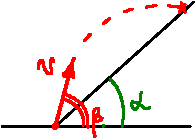
\includegraphics[width=4cm]{p09_7.pdf}}

\taskpic{ Утка летит по горизонтальной прямой с постоянной скоростью $U$. В
  неё бросил камень неопытный охотник, причём в момент броска
  скорость камня $V$ была направлена как раз на утку под углом $\alpha$ к
  горизонту. На какой высоте летела утка, если камень всё же попал в
  неё? }{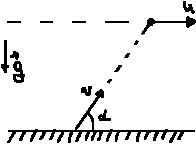
\includegraphics[width=4cm]{p09_8.pdf}}

\begin{center}
  \textsf{Листок 3.}
\end{center}
\vspace{0.01mm}
\nopagebreak[2]
\taskpic{Край гладкого горизонтального стола скруглён по окружности
  радиуса $R$. С какой наименьшей скоростью надо пустить тело, чтобы
  оно, достигнув скругления, сразу полетело по
  пораболе? }{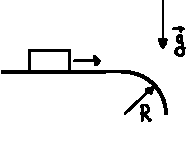
\includegraphics[width=4cm]{p09_9.pdf}}

\taskpic{По деревянным сходням, образующим угол $\alpha$ с горизонтом,
  втаскивают за привязанную к нему верёвку ящик. Коэффициент трения
  ящика о сходни $k$. Под каким углом к горизонту надо тянуть верёвку,
  чтобы с наименьшим усилием втащить ящик? }{
\begin{tikzpicture}[interface/.style={postaction={draw,decorate,decoration={border,angle=-45,amplitude=0.2cm,segment length=1.5mm}}},>=stealth]
   \draw[thick] (0.5,0) -- (3.5,3) -- ++(0,-3) -- cycle;
   \draw[thick,rotate around={45:(1.5,1)}] (1.5,1) rectangle ++(1,0.5);
   \draw[very thick,rotate around={45:(1.5,1)},->] (2.5,1.25) --
   ++(0.7,0.3);
   \draw (1.2,0) arc (0:45:0.7) node[below=0.2cm,right=0.1cm] {$\alpha$};
\end{tikzpicture}
% 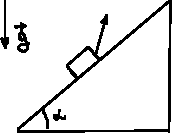
\includegraphics[width=4cm]{p09_10.pdf}
}

\taskpic{Тело массы $m_1$ лежит на доске массы $m_2$, находящейся на гладкой
  горизонтальной поверхности. Коэффициент трения между телом и доской
  $k$. Какую силу надо приложить к доске, чтобы тело соскользнуло с
  неё. За какое время тело соскользнёт, если к доске приложена сила
  $F_0$, а длина доски $l$?  }{
\begin{tikzpicture}[interface/.style={postaction={draw,decorate,decoration={border,angle=-45,amplitude=0.2cm,segment length=1.5mm}}},>=stealth]
%  \draw[help lines,step=0.5] (0,0) grid (4,4);
  \draw[interface] (0.2,0) -- ++(3.2,0);
  \draw[thick] (1,0) rectangle ++(2,0.5) node[midway] {$m_2$};
  \draw[thick] (1,0.5) rectangle ++(1,0.5) node[midway] {$m_1$};
  \draw[very thick,->] (1,0.25) -- ++(-0.5,0) node[above] {$\vec{F}_0$};
\end{tikzpicture}
%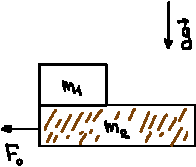
\includegraphics[width=4cm]{p09_11.pdf}
}

\taskpic{Между двумя одинаковыми гладкими брусками массами $m_1$ каждый
  вставлен клин массы $m_2$ с углом $\alpha$. Определите ускорение
  тел. }{
\begin{tikzpicture}[interface/.style={postaction={draw,decorate,decoration={border,angle=-45,amplitude=0.2cm,segment length=1.5mm}}}]
%  \draw[help lines,step=0.5] (0,0) grid (4,4);
  \draw[interface] (0.2,0) -- ++(3.6,0);
  \draw[thick] (0.5,0) rectangle ++(1,1.5) node[midway] {$m_1$}; 
  \draw[thick] (2.5,0) rectangle ++(1,1.5) node[midway] {$m_1$}; 
  \coordinate (a) at ($(1,2.25)!2!(1.5,1.5)$);
  \draw[thick] (1,2.25) -- (a) -- (3,2.25) -- cycle node[below=0.4cm,left=0.5cm]{$m_2$};
  \draw ($(a)!10pt!(3,2.25)$) arc (atan(3/2):90+atan(2/3):10pt)
  node[above=0.25cm,right=-0.05cm] {$\alpha$};
% arc (63:117:0.5) node[above=7,right] {$\alpha$};
\end{tikzpicture}
% %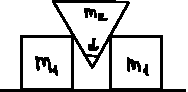
\includegraphics[width=4cm]{p09_12.pdf}
}

\begin{center}
  \textsf{Листок 4.}
\end{center}
\vspace{0.01mm}
\hrule

\task{К свободному концу нити, прикреплённой к стене и перекинутой
  через блок, подвешен груз. Блок закреплён на бруске массы $m_0$,
  который может скользить по горизонтальной плоскости без трения. В
  начальный момент нить с грузом отклоняют от вертикального положения
  на угол $\alpha$ и затем отпускают. Определите ускорение бруска, если
  угол, образованный нитью с вертикалью, не меняется при движении
  системы. Чему равна масса груза.  }

\task{Где находится центр масс: однородного прута, согнутого
  посередине под прямым углом; однородной треугольной пластинки;
  гардеробного номерка в виде диска с круглым отверстием.  }

\task{ Обезьяна массы $m$ уравновешена противовесом на блоке $А$. Блок $А$
  уравновешен грузом массы $2m$ на блоке $В$. Система неподвижна. Как
  будет двигаться груз, если обезьяна начнёт равномерно выбирать
  верёвку со скоростью $V$ относительно себя? Массой блоков и трением
  пренебречь.}

\task{ С какой силой давит на землю кобра, когда она, готовясь к
  прыжку, поднимается вертикально вверх с постоянной скоростью $V$?
  Масса змеи $m$, её длина $l$.  }

\begin{center}
  \textsf{Листок 5.}
\end{center}
\vspace{0.01mm}
\hrule

\task{Автомобиль с работающим д вигателем въезжает на обледенелую
  гору, поверхность которой образует угол $\alpha$ с горизонтом. Какой
  высоты гору может преодолеть автомобиль, если его начальная скорость
  при въезде на него равна $V$, а коэффициент трения колёс о лёд $k$?}

\task{Каков радиус орбиты спутника, лежащей в экваториальной
  плоскости, если тот всё время находится в зените над одной и той же
  точкой земной поверхности?  }

\task{Однородный куб с помощью верёвки, привязанной к середине его
  ребра, подвешен к вертикальной стене. При каких значениях угла
  между верёвкой и стеной куб соприкасается со стеной всей гранью,
  если коэффициент трения его о плоскость равен $k$?}

\task{Лестница опирается на вертикальную стену и пол. При каких
  значениях угла между лестницей и полом она может стоять если
  коэффициент трения лестницы о пол и о стену равен $k_1$ и $k_2$
  соответственно?}

\begin{center}
  \textsf{Листок 6.}
\end{center}
\vspace{0.01mm}
\nopagebreak[2]
\task{Необходимо с поверхности земли попасть камнем в цель, которая
  расположена на высоте $h$ и на расстоянии $S$ по горизонтали. При какой
  наименьшей скорости это возможно? Сопротивлением воздуха пренебречь.}

\task{Между целью и миномётом, находящимся на одной горизонтали,
  расположена стена высотой $h$. Расстояние от стены до миномёта $a$, от
  стены до цели $b$. Определить минимальную начальную скорость мины,
  необходимую для поражения цели. Под каким углом при этом надо
  стрелять? Сопротивлением воздуха пренебречь.  }

\task{Гладкий однородный стержень длины $2L$ опирается на край
  полусферической чаши радиуса $R$. Какой угол с горизонтом образует
  стержень в положении равновесия?}

\task{Зенитное орудие может сообщить снаряду скорость $V$ в любом
  направлении. Требуется найти зону поражения, т. е. границу,
  отделяющую цели, до которых снаряд из данного орудия может долететь,
  от недостижимых целей. Сопротивлением воздуха пренебречь.}

\task{Автомобиль удаляется от стены со скоростью $V$ под углом $\alpha$ к
  ней. В момент, когда расстояние до стены равно $l$, шофёр подаёт
  короткий звуковой сигнал. Какое расстояние пройдёт автомобиль до
  момента, когда шофёр услышит эхо? Скорость звука в воздухе $c$.}

%%% Local Variables: 
%%% mode: latex
%%% TeX-master: "../../../report"
%%% End: 

\begin{center}
  \textsf{Листок 7.}
\end{center}
\vspace{0.01mm}
\nopagebreak[2]

\taskpic{ 
Два одинаковых кубика с длиной ребра $b$ массой $m$ каждый
  стоят на горизонтальном столе, на расстоянии $b$ друг от друга. Между
  ними помещён рычаг длиной $2^{3/2}b$ с пренебрежимо малой
  массой. Коэффициент трения между поверхностями кубиков и столом
  $k$. Коэффициент трения между рычагом и кубиками очень большой в точке
  $A$ и очень маленький в точке $C$. В точке $B$ приложена сила $F$,
  направленная перпендикулярно рычагу как показано на
  рисунке. Определите, какой из кубиков сдвигается раньше, если
  постепенно увеличивать силу $F$.  }
{ 
\begin{tikzpicture}[>=stealth,scale=0.45]
    \draw (-0.4,0) -- (6.4,0);
    \draw[brown,thick] (0,0) rectangle ++(2,2) ++(2,-2) rectangle ++(2,2);
    \coordinate (a) at (2,0);
    \coordinate (f) at ($(a)!5.6!45:(3,0)$);
    \draw[thick] (a) -- (f);
    \draw[->] (f) -- ++(-45:1) node[below] {$\vec{F}$};
  \end{tikzpicture}
%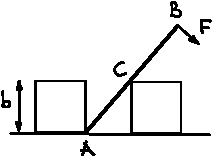
\includegraphics[width=4cm]{p09_26.pdf}
}

\taskpic{ Однородный стрежень длиной $l$ опирается о пол и
  ступеньку. Коэффициент трения между стержнем и полом равен 1, трения
  между стержнем и ступенькой нет. При какой высоте ступеньки стержень
  может находиться в равновесии, если угол $\alpha = \pi /4$?
}{\begin{tikzpicture}[>=stealth,scale=1]
\draw (-0.5,3) -- (0,3) -- (0,0) -- (3.3,0);
\draw[brown, very thick] (3,0) -- +(135:5) node[black,midway, above] {$l$};
\draw[black] (3,0) +(135:0.5) arc (135:180:0.5);
\path (3,0) + (160:0.7) node{$\alpha$};
\draw[thick,->] (2.7,3) -- (2.7,2.5);
\path (3,2.7) node {$\vec{g}$};
\end{tikzpicture}
%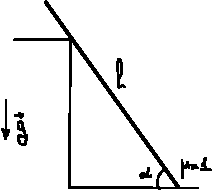
\includegraphics[width=4cm]{p09_27.pdf}
}

\taskpic{ В системе, изображённой на рисунке, трение в блоках и между
  другими поверхностями отсутствует. Если грузу массой $m$ позволить
  двигаться, то за какое время он достигает подставки? Начальная
  скорость груза равна нулю, начальное расстояние от груза до
  подставки $h$, нить невесомая и нерастяжимая. Масса подставки $M$.
}{
\begin{tikzpicture}[>=stealth,scale=0.6]
  \draw (-0.3,0) -- ++(5.3,0) -- ++ (0,5);
  \draw[thick] (0,0) rectangle (2,1) node[midway] {$M$};
  \draw[thick] (0,1) rectangle (1,5);
  \draw (2,0.5) -- (4.6,0.5);
  \filldraw[white,draw=black] (4.6,0.7) circle (0.2);
  \draw (4.6,0.7) -- ++(0.4,-0.3);
  \draw (4.8,0.7) -- ++(0,3.6);
  \filldraw[white,draw=black] (4.6,4.3) circle (0.2);
  \draw (4.6,4.3) -- ++(0.4,0);
  \draw (4.6,4.5) -- ++(-3.2,0);
  \filldraw[white,draw=black] (1.4,4.3) circle (0.2);
  \draw (1.4,4.3) -- ++(-0.4,0.3);
  \draw (1.2,4.3) -- ++(0,-1);
  \draw[thick] (1,3.3) rectangle ++(0.4,-0.4) node[above=0.3cm,right]
  {$m$};
  \draw[dashed] (0,1) -- ++(-0.5,0) ++ (0,2.1) -- ++(1.7,0);
  \draw[thick,<->] (-0.3,1) -- ++(0,2.1) node[midway,left] {$h$};
\end{tikzpicture}
%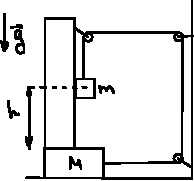
\includegraphics[width=4cm]{p09_28.pdf}
}

\taskpic{ Найдите ускорение грузов, если масса каждого груза равна
  $m$. Массами нитей и блоков пренебречь, нити нерастяжимы, трение
  отсутствует.
}{
\begin{tikzpicture}[scale=0.6]
  \draw (1,0) -- (5,0) (3,0) -- (3,-1.5);
  \filldraw[thick,white,draw=black] (3,-1.5) circle (0.9);
  \draw (2.1,-1.5) -- ++(0,-2) (3.9,-1.5) -- ++(0,-3);
  \filldraw[thick,white,draw=black] (2.1,-3.5) circle (0.6);
  \filldraw[thick,white,draw=black] (3.3,-4.5) circle (0.6);
  \draw (2.7,-3.5) -- +(0,-1);
  \draw (2.1,-3.5) -- +(0,-2.5);
  \draw (3.3,-4.5) -- +(0,-1.5);
  \node [rectangle,fill=white,draw=black,minimum height=0.7,thick] at
  (2.1,-6) {$m$};
  \node [rectangle,fill=white,draw=black,minimum height=0.7,thick] at
  (3.3,-6) {$m$};
\end{tikzpicture}
%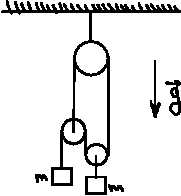
\includegraphics[width=4cm]{p09_29.pdf}
}

\setcounter{notask}{1}
\parindent=5mm

\subsubsection{Экспериментальные работы.}
\label{sec:daily_9_exp}

\textsf{Преподаватель: А.В.\,Лиознова.}

\begin{enumerate}
\item Измерить толщину масляной плёнки. \\ \textit{Оборудование:} шприц, масло, линейка.
\item Найти неизвестное сопротивление. \\ \textit{Оборудование:} вольтметр, батарейка, сопротивление, провода.
\item Измерить силу разрыва нити. \\ \textit{Оборудование:} нитки, кнопки, грузики.
\item Найти показатель преломления жидкости. \\ \textit{Оборудование:} лазерная указка, линейка, бумага, пластиковые стаканчики.
\item Измерить отношение коэффициента трения покоя к коэффициенту
  трения скольжения дерева по дереву. \\ \textit{Оборудование:} деревянный брусок, палочка, линейка.
\item Измерение скорости муравья.  \\ \textit{Оборудование:} линейка,
  секундомер, муравей.
\item Определить содержание соли в воде. \\ \textit{Оборудование:}
  прозрачная бутылка, пластилин, вода с солью, колпачок от ручки.
\item Определить плотность металла в пластилине. \\
  \textit{Оборудование:} разновесы, пластилин с металлом, стакан с
  водой.
\item Исследование времени падения тел различной массы. \\
  \textit{Оборудование:} грузики, секундомер.
\item Нахождение центра масс тела неправильной формы. \\
  \textit{Оборудование:} линейка, нитки, неизвестное тело (вырезано из
  картона).
\end{enumerate}

\subsection{10 класс.}
\label{sec:daily_10}

\subsubsection{Теория.}
\label{sec:daily_10_th}

\textsf{Преподаватель: С.С.\,Колеватов.}
\smallskip

В 10 классе лекции были посвящены электростатике. Выбор такого
предмета лекций неслучаен: многолетний опыт работы в жюри физических
олимпиад показывает, что школьники зачастую относятся к электростатике
как к набору простейших формул, не понимая физического смысла
явлений. В школьном курсе физики, по нашим наблюдениям, электростатика
была и остаётся одним из самых сложных разделов.

После окончания курса электростатики был прочитан мини–курс по
гидродинамике. Поскольку математический аппарат был довольно схож с
аппаратом электростатики, удалось разобрать довольно большое число
физических явлений, не выводя заново математические факты, а пользуясь
лишь электромеханическими аналогиями. Такой подход, кроме всего
прочего, хорошо демонстрирует единство методов, применяемых в физике. 

\begin{center}
  \textsf{План занятий.}
\end{center}

\begin{enumerate}
\item История.  Закон Кулона. 2 вида зарядов.  Принцип
  суперпозиции. Независимость парных взаимодействий, дискретность
  заряда. Закон сохранения заряда. Напряженность электрического
  поля. Электрическое поле точечного заряда, системы точечных зарядов.
  Линии векторного поля. Поток вектора электрического поля.
  Электростатическая теорема Гаусса и её доказательство.
\item Свойства линий электрического поля. Теорема Ирншоу и её
  доказательство. Задачи на применение теоремы Гаусса.
  Потенциальность кулоновских сил. Электростатические и гравитационные
  силы. Потенциальная энергия. Потенциал. Потенциал точечного заряда.
\item Производная. Частная производная. Градиент. Связь потенциала с
  напряженностью электрического поля. Краевая задача
  электростатики. Задача Дирихле. Задача Неймана. Краевая задача с
  границей в виде проводника.  Проводники. Определение. Свойства
  проводников. Экранирование.
\item Метод изображений. Решение задач с помощью метода изображений.
  Заряд и заземленная плоскость, заземленных уголок, сфера.
  Электростатическая емкость уединенного проводника. Емкость шара.
\item Емкость конденсатора.Плоский конденсатор.Соединение
  конденсаторов. Энергия взаимодействия зарядов. Энергия
  конденсатора. Электрический ток. Сила тока. Плотность тока. Закон
  Ома. Сопротивление. Соединение сопротивлений.
\item Проводимость. Вывод зависимости сопротивления от проводимости и
  размеров тела. Закон Ома в дифференциальной форме. Правила
  Кирхгофа. Алгоритм и пример решения задач. Закон Джоуля-Ленца и его
  доказательство. Сверхпроводники. Высокотемпературная
  сверхпроводимость.
\item Эффект Пельтье. Энергетические уровни. Эффект
  Томсона. Термопара. Градуировка термопары. Решение схем~---~метод
  контурных токов, метод эквивалентной э.д.с.
\smallskip
\hrule
\item Гидродинамика. Основные определения. Приближения, в которых
  будут выписываться уравнения. Линии тока, их свойства, связь с
  силовыми линиями. Уравнение неразрывности. Поток через малый
  куб. Запись уравнения аналогично теореме Гаусса. Уравнение Бернулли.
\item Вязкость. Формула Пуазейля (распределение скоростей в
  круглой трубе с жидкостью, поток воды через трубу в единицу
  времени).
\item Вязкость или турбулентность? Коэффициент сопротивления и число
  Рейнольдса. Поверхностное натяжение: поверхностный слой, его
  энергия. Оценка радиуса капли в момент отрыва.

\end{enumerate}

\subsubsection{Решение задач.}
\label{sec:daily_10_problems}

\textsf{Преподаватель: Д.С.\,Смирнов.}
\smallskip

Программа задач по теме «Электростатика» призвана дополнять курс
теоретических лекций. Программа разработана таким образом, что
сложность задач от занятия к занятию постепенно увеличивается. Это
позволяет школьникам начать с простых и увлекательных задач, а затем
повысить своё мастерство до уровня численного описания сложных
физических экспериментов и расчёта некоторых электротехнических
схем. Контрольная, проведённая по итогам темы «Электростатика»,
показала, что слушатели успешно усвоили материал занятий. На последних
занятиях школьники познакомились с гидродинамикой.

Кроме того, на занятиях, прошедших после физбоёв, разбирались задачи,
вызвавшие особое затруднение у школьников. 

Ниже приводятся задачи, обсуждавшиеся на занятиях. Большинство из них
взято из классического задачника повышенной сложности под редакцией
О.Я.~Савченко. 

\begin{center}
  \textsf{Листок 1.}
\end{center}
\vspace{0.01cm}
\nopagebreak[2]
\task{Что будет происходить, если потереть стеклянную палочку о шёлк и
  затем подносить её к бумажному шарику на шёлковой нити? А затем
  коснуться палочкой второго такого же шарика? А затем сблизить
  шарики?}
\task{Как будут меняться показания электроскопа, если трижды коснуться
  его наэлектризованной палочкой?}
\task{Что произойдёт, если соединить два электроскопа: один
  заряженный, а другой нет медной проволокой, держа её в руках? Держа
  её на подвесе из шёлковых нитей? Если соединить те же электроскопы
  чёрной, белой или шёлковой нитью?}
\task{Что будет, если нагреть конец заряженного электроскопа?}
\task{Что будет происходить в последовательном соединении лампочки,
  батарейки и стеклянной трубочки, если последнюю постепенно
  нагревать?}
\task{Что будет, если зарядить один электроскоп стеклянной палочкой
  потёртой о шёлк, другой сургучом потёртым о шерсть, а затем
  соединить их проволокой?}
\task{Как будет вести себя заряженный груз, подвешенный на нити, если
  приближать к нему руку?}

\begin{center}
 \textsf{Листок 2.}
\end{center}
\vspace{0.01cm}
\nopagebreak[2]
\task{Чему равно электрическое поле на оси равномерно заряженной
  сферы, у которой удалили узкий поясок вблизи экватора?}
\task{Сила взаимодействия между двумя одинаковыми зарядами на
  расстоянии 1 м равна 1 Н. Определите эти заряды в СИ и СГС.}
\task{Предположим, что удалось бы разъединить 1 $\mbox{см}^3$ воды на
  элементарные разноимённые заряды, которые затем удалили бы друг от
  друга на расстояние 100 км. С какой силой притягивались бы эти
  заряды?}
\task{На концах горизонтальной трубы длины $l$ закреплены
  положительные заряды $q_1$ и $q_2$. Найдите положение равновесия
  шарика с положительным зарядом $q$, который помещён внутрь
  трубы. Устойчиво ли это положение равновесия? Будет ли положение
  равновесия отрицательно заряженного шарика устойчивым?}
\task{В атоме водорода электрон движется вокруг протона с угловой
  скоростью $10^{16}$ рад/с. Найдите радиус орбиты.}
\task{Чему равна напряжённость электрического поля в центре равномерно
заряженного тонкого кольца радиуса $R$? Чему она равна на оси кольца
на расстоянии $h$ от центра? Заряд кольца $Q$. }
\task{
  Металлическое кольцо разорвалось кулоновскими силами, когда заряд
  кольца был равен $Q$. Сделали точно такое же новое кольцо, но из
  материала, прочность которого в 10 раз больше. Какой заряд разорвёт
  новое кольцо? 
}


%%% Local Variables: 
%%% mode: latex
%%% TeX-master: "../../../report"
%%% End: 

\begin{center}
 \textsf{Листок 3.}
\end{center}
\vspace{0.01cm}
\hrule
\parindent=0mm

\task{
  Напряжённость однородного электрического поля равна $E$. Чему равен
  поток напряжённости электрического поля через квадрат со стороной
  $l$, плоскость которого расположена под углом $30^{o}$ к направлению
  поля? 
}
\task{
  Найдите отрицательные и положительные потоки однородного
  электрического поля напряжённости $E$ через замкнутую поверхность
  прямой трёхгранной призмы, высота которой $h$. Передняя грань
  призмы, ширина которой равна $h$, перпендикулярна $E$, нижняя грань
  параллельна $E$. 
}
\task{Используя теорему Гаусса, определите напряжённость
  электрического поля внутри и вне равномерно заряженной сферы, если
  полный заряд сферы $Q$; равномерно заряженной бесконечной нити, если
  заряд единицы длины равен $\rho$; вне и внутри равномерно заряженной
  бесконечной пластины толщиной $h$, если объёмная плотность заряда в
  пластине равна $\rho$.}
\task{
  Докажите теорему Ирншоу. 
}
\task{
  При пересечении двух шаров радиуса $R$, центры которых находятся на
  расстоянии $l$ друг от друга, образуются два <<полумесяца>>,
  равномерно заряженных разноимёнными электрическими
  зарядами. Объёмная плотность электрического заряда равна
  $\rho$. Докажите, что электрическое поле в области пересечения шаров
  однородно. Найдите его напряжённость. 
}

\taskpic{В равномерно заряженной бесконечной пластине вырезали
  сферическую полость так, как показано на рисунке. Толщина пластины
  $h$, объёмная плотность заряда $\rho$. Чему равна напряжённость
  электрического поля в точке $A$, в точке
  $B$?}{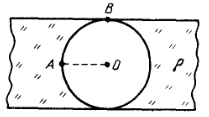
\includegraphics[width=4cm]{d10_3_1.png}}
\task{
  Две пересекающиеся под углом $\alpha$ бесконечные плоскости делят
  пространство на четыре области. Чему равна напряжённость
  электрического поля в этих областях, если поверхностная плотность
  заряда плоскостей $\pm \sigma$?
}
\begin{center}
 \textsf{Листок 4.}
\end{center}
\vspace{0.01cm}
\nopagebreak[2]
\task{Потенциал заряженного проводника 300 В. Какой минимальной
  скоростью должен обладать электрон, чтобы улететь с поверхности
  проводника на бесконечно далёкое от него расстояние?}

\task{
  Заряд 0.1 Кл удалён от заряда 0.2 Кл на расстояние 20 м. Чему равен
  потенциал поля в середине отрезка, соединяющего заряды? 
}

\task{
  Заряды 100, 10, 1, -10, -1, -10 СГС находятся в вершинах правильного
  шестиугольника со стороной 2 см. Чему равен потенциал в центре
  шестиугольника в СИ и СГС? 
}

\task{
  Две бесконечные проводящие изолированные плиты заряжены так, что
  суммарная поверхностная плотность заряда обеих сторон первой плиты
  равна $\sigma_1$, а второй --- $\sigma_2$. Плиты параллельны друг
  другу. Найдите поверхностную плотность заряда на каждой стороне
  плит. 
}

\task{
  Найдите напряжённость электрического поля между тремя пластинами в
  случае, если средняя пластина заземлена. Расстояния между средней
  пластиной и крайними $a$ и $b$. Потенциал крайних пластин $\phi$. 
}

\task{
  В полости металлического шара радиуса $R$ находится заряд
  $Q$. Найдите заряд, индуцируемый этим зарядом на поверхности
  полости. Почему на поверхности шара заряд будет распределён с
  постоянной плотностью? 
}

\task{
  Металлический шар радиуса $R_1$, заряженный до потенциала $\phi$,
  окружают концентрической проводящей незаряженной оболочкой радиуса
  $R_2$. Чему станет равен потенциал шара, если заземлить оболочку?
  Соединить шар с оболочкой проводником? 
}
\begin{center}
 \textsf{Листок 5.}
\end{center}
\vspace{0.01cm}
\hrule
\parindent=0mm

\task{
  Размеры пластин плоского конденсатора увеличили в два раза. Как
  изменилась его ёмкость? Как изменится ёмкость, если расстояние между
  пластинами удвоить? 
}

\task{
  Определите ёмкость конденсатора, образованного двумя
  концентрическими сферами радиуса $R_1$ и $R_2$.
}

\task{
  Определите ёмкость систем конденсаторов, изображённых на рисунке. 
}

\task{
  Как изменится ёмкость плоского конденсатора, если поместить его в
  металлическую коробку? Расстояние от обкладок до стенок коробки
  равно расстоянию между обкладками $d$. Как изменится ёмкость, если
  коробку соединить с одной из обкладок? 
}

\begin{center}
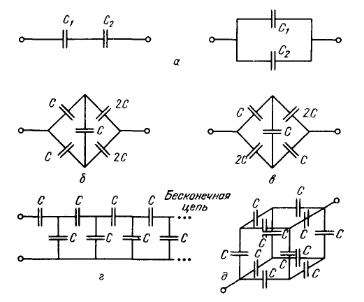
\includegraphics[scale=0.6]{d10_5_1.png}  
\end{center}


\begin{center}
 \textsf{Листок 6.}
\end{center}
\vspace{0.01cm}
\hrule
\parindent=0mm

\task{
  Определите силу, с которой притягиваются друг к другу пластины
  плоского конденсатора, если источник тока, зарядивший конденсатор до
  разности потенциалов 1000 В, отсоединён. Площадь пластин 100
  $\mbox{см}^2$, расстояние между пластинами 1 мм. Изменится ли сила
  взаимодействия пластин, если источник тока будет постоянно
  подсоединён к пластинам?
}

\task{
  Как изменится энергия конденсатора, если при той же разности
  потенциалов между пластинами увеличить все его геометрические размеры
  в $k$ раз?
}

\task{
  На пластины плоского конденсатора помещён заряд $Q$. Площадь пластин
  $S$, расстояние между ними $d$. Какую работу надо совершить, чтобы
  увеличить расстояние между пластинами на $d$? Какую работу надо
  совершить, чтобы сдвинуть пластины на расстояние $x$ относительно
  друг друга? Пластины имеют форму квадрата со сторой $a$. Какая
  совершается работа в обоих предыдущих случаях, если между пластинами
  конденсатора поддерживается батареей постоянная разность
  потенциалов? 
}


\begin{center}
 \textsf{Листок 7 (гидродинамика).}
\end{center}
\vspace{0.01cm}
\nopagebreak[2]
\task{ Под каким углом к горизонту располагается вода в сосуде,
  движущемся с известным ускорением?  }

\task{ Под каким углом к полу вагона расположится чай в стакане, если
  поезд движется по окружности радиусом 1 км со скоростью 72 км/ч ?  }

\task{ С какой скоростью вытекает вода через маленькую дырочку у дна
  широкой бочки с известным уровнем воды? А из узкой бочки, если
  известны площади бочки и дырки? Что изменится, если дырка не в боку,
  а в дне?}

\task{ Как меняется площадь сечения струи, вытекающей из крана, с
  высотой?  }

\task{ Как определить, в какую сторону действует подъёмная сила на
  крыло известной формы? }

\task{ Даны времена, за которые параллелепипедовидная ванна известных
  размеров наполняется из крана и опустошается через дырку в дне. До
  какой высоты дойдёт вода, если одновременно открыть и кран, и дырку?
}

%%% Local Variables: 
%%% mode: latex
%%% TeX-master: "../../../report"
%%% End: 

\begin{center}
 \textsf{Листок 8 (заключительная контрольная).}
\end{center}
\vspace{0.01cm}
\hrule
\parindent=0mm

\task{
  Два одинаковых заряженных шарика массы $m$, подвешенных в одной
  точке на нитях длины $l$, разошлись так, что угол между нитями стал
  прямым. Определите заряд шариков. 
}

\task{Чему равен поток напряжённости однородного электрического
  поля через боковую поверхность усечённого конуса, радиусы сечения
  которого равны $R$ и $r$? Напряжённость электрического поля $E$
  составляет угол $\alpha$ с осью конуса. }

\task{
  Три проводящие концентрические сферы радиуса $r$, $2r$, $3r$ имеют
  заряд соответственно $q$, $2q$, $-3q$. Определите потенциал на
  каждой сфере.
}

\task{ Какие заряды индуцируются на каждом из трёх одинаковых
  конденсаторов ёмкости $C$, соединённых звездой, если подать на
  свободные концы напряжения 0, $\phi$ и $2\phi$?  }

\setcounter{notask}{1}

\parindent=5mm

\subsubsection{Экспериментальные работы.}
\label{sec:daily_10_exp}

\textsf{Преподаватель: А.Г.\,Кострыгин.}

\begin{enumerate}
\item Измерить модуль упругости каучукового шарика. \\
  \textit{Оборудование:} каучуковый шарик, вода, линейка.
\item Измерить атмосферное давление. \\ \textit{Оборудование:} вода, трубочки, линейка.
\item Распределение Гаусса. \\ \textit{Оборудование:} монетки.
\item Измерение диаметра выходного отверстия у шприца. \\
  \textit{Оборудование:} шприц, линейка.
\item Измерение радиуса песчинки. \\ \textit{Оборудование:}
  секундомер, линейка.
\item Изучение зависимости силы растяжения резинки от её удлинения. \\
  \textit{Оборудование:} миллиметровка, резинка, линейка, грузики.
\item Измерение отношения длин ниток маятника. \\ \textit{Оборудование:} нитки,
  грузики.
\item Нахождение хаусдорфовой размерности листа дерева. \\
  \textit{Оборудование:} лист клёна, линейка.
\item Измерение скорости вытекания воды из крана. \\
  \textit{Оборудование:} линейка.
\item Измерение плотности карандаша. \\ \textit{Оборудование:} вода,
  нитки, линейка, карандаш. 
\end{enumerate}

\subsection{11 класс.}
\label{sec:daily_11}

\subsubsection{Теория.}
\label{sec:daily_11_th}

\textsf{Преподаватель: И.Е.\,Шендерович.}
\smallskip

В 11 классе лекции были посвящены электродинамике. Последние два
занятия были посвящены применению общей теории к анализу электрических
цепей переменного тока, а также кратко изучалась волновая оптика. 

Целью такого курса было изучение разнообразных методов, широко
применяемых в физике. Кроме того, итогом лекций явилось построение
цельной самосогласованной теории, различные следствия которой можно
наблюдать на эксперименте. Фактически, школьники в первый раз
столкнулись с построением работающей физической теории из
первопринципов (в данном случае за основу были взяты законы
сохранения). 

\begin{center}
  \textsf{План занятий.}
\end{center}

\begin{enumerate}
\item Физические принципы электродинамики. Понятие о физических
  полях. Примеры полей: поле температур, поле скоростей. Скалярные и
  векторные поля. Основные операции с векторами. Начала векторного
  анализа. Интегральные теоремы векторного анализа. Теорема Стокса,
  Гаусса–Остроградского.
\item Электростатика. Закон Кулона как следствие теоремы
  Гаусса. Потенциал как следствие безвихревой природы электрического
  поля. Уравнение Пуассона. Теорема Ирншоу.
\item Энергия электрического поля. Аналогии с гидродинамикой (задача
  об обтекании шара идеальной жидкостью) и теплопроводностью
  (распределение температур в среде с простой геометрией).
\item Сохранение энергии в электродинамике. Связь закона сохранения
  энергии и уравнений Максвелла. Получение уравнений Максвелла, их
  физический смысл. Симметрия в уравнениях Максвелла. Калибровка.
\item Частный случай: магнитостатика. Закон Био–Савара–Лапласа, закон
  Ампера. Примеры применения этих законов, расчёт магнитного поля от
  проводников с током простой формы.
\item Физика индукции. Закон Фарадея. Сила Ампера. Задача про
  взаимодействие параллельных токов. Сила Лоренца. Два источника
  возникновения магнитного поля, физический смысл этого.
\item Движущееся электромагнитное поле. Задача про движущуюся
  заряженную плоскость. Понятие об электромагнитной волне. Волновые
  процессы в электродинамике. Волновое уравнение.
\item Задача про конденсатор в переменном электрическом поле. Пример
  решения физической задачи методом последовательных
  приближений. Функция Бесселя.
\item Законы Кирхгофа. Примеры применения законов Кирхгофа к цепям
  постоянного и переменного тока. Катушки индуктивности. Аналогия с
  механикой. Колебательный контур.
\item Понятие о волновой оптике. Явление интерференции как следствие
  волновой природы света. Интерференция от двух точечных источников
  света. Интерференция на плоскопараллельной пластинке.
\end{enumerate}

\subsubsection{Решение задач.}
\label{sec:daily_11_problems}

\textsf{Преподаватель: Д.В.\,Батькович.}
\smallskip

\subsubsection{Экспериментальные работы.}
\label{sec:daily_11_exp}

\textsf{Преподаватель: Я.Ю.\,Коптелов.}
\smallskip

Экспериментальные задачи в 11 классе в большинстве своём состояли из
задач, ранее предлагавшихся на городских и Всероссийских
олимпиадах. Почти в каждой задаче для того, чтобы измерить требуемую
величину с помощью предлагающегося оборудования, школьник должен был
придумать оригинальную методику. Кроме экспериментов по стандартной
школьной программе, в программу 11 класса были включены эксперименты
по интерференции и дифракции (№7, №10), по гидродинамике (№5), а также
по теории колебаний (№9).

\begin{enumerate}
\item Изучение зависимости силы сопротивления среды от скорости. \\
  \textit{Оборудование:} теннисные шарики, нитка, линейка.
\item Изучение распределения вероятностей нахождения груза в
  математическом маятнике. \\ \textit{Оборудование:} нитки, груз.
\item Измерение толщины масляного пятна на поверхности воды. \\
  \textit{Оборудование:} масло, вода, линейка.
\item Измерение массы куска пластилина. \\ \textit{Оборудование:}
  карандаш, вода, нитка, линейка.
\item Измерение радиуса песчинки. \\ \textit{Оборудование:} вода, секундомер.
\item Измерение момента инерции шарика. \\ \textit{Оборудование:}
  каучуковый шарик, вода, линейка.
\item Измерение объёма данных на компакт--диске. \\
  \textit{Оборудование:} компакт--диск, указка, линейка.
\item Измерение плотности карандаша. \\ \textit{Оборудование:} вода,
  нитки, линейка, карандаш.
\item Исследование колебательных мод в двойном маятнике. \\
  \textit{Оборудование:} нитки, монетки.
\item Измерение длины волны лазерной указки. \\ \textit{Оборудование:}
  фольга, булавки, указка, линейка.
\end{enumerate}

\subsection{Факультативы.}
\label{sec:elective}

Каждый рабочий день в ЛФШ проводились факультативы, или
спецкурсы. Спецкурсы обычно представляют собой серию из 4-5 лекций по
1 часу, по теме, не входящей в школьную программу. Целью подобных
спецкурсов является рассказ об области науки, являющейся новой и
неизвестной для школьников. Школьники свободны в выборе спецкурсов для
посещения.

\begin{center}
\textsf{Список прочитанных спецкурсов.}  
\end{center}

\begin{enumerate}
\item Космология. \\ \textsf{Преподаватель: С.С.\,Колеватов.}

  Общая теория относительности. Модель Фридмана. Космологическая
  постоянная. Сжимающаяся или расширяющаяся Вселенная. Большой
  Взрыв. Элементарные частицы в первые три минуты. Тёмная материя и
  тёмная энергия.

\item Физика элементарных частиц. \\ \textsf{Преподаватель: И.Е.\,Шендерович}.

  Шкала энергий в физике частиц. Материя. Классификация элементарных
  частиц. Бозоны и фермионы. Виды фундаментальных взаимодействий. Роль
  симметрии в физике частиц. Законы сохранения и их
  нарушения. Античастицы. Странность и изоспин. Кварковая модель. Цвет
  и аромат.

\item Квантовая механика. \\ \textsf{Преподаватель: И.А.\,Барыгин}.

  Волны. Явление интерференции. Электромагнитные волны. Внешний
  фотоэффект. Фотон. Опыт с двумя щелями. Дебройлевская длина
  волны. Принцип неопределённости.

\item Полупроводники.  \\ \textsf{Преподаватель: Д.С.\,Смирнов}.

  Металлы, диэлектрики, полупроводники. Собственные
  полупроводники. Примесные полупроводники. Язык энергетических
  диаграмм. Рождение и смерть электрона и дырки. Тепловое
  движение. Барьер на границе кристалла. Работа выхода. Поверхностное
  состояние. Поверхностный потенциал. 

\item Эксперименты в физике частиц.  \\ \textsf{Преподаватель: Р.С.\,Колеватов}.
\item Хаос и фракталы.\\ \textsf{Преподаватель: И.Е.\,Шендерович}.

  Общее понятие о хаосе. Логистическое отображение. Бифуркационная
  диаграмма. Удвоение периода. Критическое значение
  параметра. Постоянная Фейгенбаума. Универсальность. Отображение
  Жюлиа. Множество Мандельброта. Хаос в физических системах. Маятник с
  колеблющейся точкой подвеса. Магнетизм. Идея перенормировки на
  примере фазового перехода в точке Кюри. Наличие хаотической динамики
  вблизи точки Кюри.

\item Теория узлов. \\ \textsf{Преподаватель: А.М.\,Минарский}. 
\item Психология. \\ \textsf{Преподаватель: Н.В.\,Тараканов}. 
\item История Великой Отечественной Войны. \\

  Рассматривались основные сражения и операции во время ВОВ. Каждое
  занятие факультатива представляло собой подробный рассказ о
  каком-либо временном этапе с июня 1941 года по август 1945
  года. Было проведено десять семинаров, в подготовке занятий
  участвовали все преподаватели.
\end{enumerate}

\subsection{Физические бои.}
\label{sec:battles}

Физические бои проходили по классам. Жюри выбирало капитанов, которые
могли самостоятельно набирать команду по системе, принятой в
футбольных соревнованиях. Таким образом, соревнующиеся команды были
примерно одинаковой силы.

В 8 классе был проведён один физбой (участвовало 8 человек, две
команды). В 9 классе был также проведён один физбой (участвовало 15
человек, три команды). В 10 и 11 классе физбои проводились в два дня
(полуфинал и финал), участвовало 21 и 23 человека соответственно
(по четыре команды в каждом классе). 

Задачи для физбоёв подбирались в основном из сборников задач повышенной
сложности, а также из всевозможных физических олимпиад. Использовалась
следующая литература: 

\begin{enumerate}
\item <<Всероссийские олимпиады по физике 1992-2001>>, сборник задач
  под ред. С.М.\,Козела и В.П.\,Слободянина. М., 2002.
\item <<Олимпиадные задачи по физике. Международная олимпиада
  ``Туймадаа''>>, под ред. Ю.М.\,Григорьева, В.М.\,Муравьёва,
  В.Ф.\,Потапова. М., 2007.
\item <<Польские физические олимпиады>>, В.\,Горшковский. М., 1982.
\item Задачи из журнала <<Квант>>, 1970--2006. 
\item <<Задачи Московских физических олимпиад>>, под ред.
  С.С.\,Кротова. М., 1988.
\item 1001 задача по физике с решениями, И. М.\,Гельфгат, 
  Л.Э.\,Генденштейн, Л.А.\,Кирик. Харьков--Москва, 1996.
\end{enumerate}

Ниже приводятся задачи, выдававшиеся на физбоях. 

% \newgeometry{top=1cm,bottom=1cm,left=1.5cm,right=1.5cm}

% \begin{center}
 \textsc{Физбой, 7--8 классы.}
\end{center}
\vspace{0.01cm}
\hrule
\parindent=0mm

\task{Легкая пружина длины $l$, жесткости $k$ установлена на столе
  вертикально. На нее падает небольшой шарик массой $m$. Определите,
  на какой высоте $h$ от поверхности стола шарик будет иметь
  максимальную скорость.}

\task{На пробку массой $m_{\mbox{\textit{пр}}}$ намотана проволока из
  алюминия. Плотность пробки равна $\rho_{\mbox{\textit{пр}}} =
  0{,}5\cdot10^3\mbox{ кг/м}^3$, алюминия $\rho_{\mbox{\textit{ал}}} =
  2{,}7\cdot10^3\mbox{ кг/м}^3$, воды $\rho_{\mbox{\textit{в}}} =
  1\cdot10^3\mbox{ кг/м}^3$. Определите, какую минимальную массу
  $m_{\mbox{\textit{ал}}}$ проволоки надо намотать на пробку, чтобы
  пробка вместе с проволокой полностью погрузилась в воду.}

\taskpic{К концу однородной палочки массой $M = 4{,}4\mbox{ г}$
  подвешен на невесомой нити однородный алюминиевый шарик радиуса $r =
  0{,}5\mbox{ см}$. Палочку кладут на край стакана с водой, добиваясь
  такого положения равновесия, при котором погруженной в воду окажется
  половина шарика. Плотность алюминия равна $\rho_{\mbox{\textit{ал}}}
  = 2{,}7\cdot10^3\mbox{ кг/м}^3$, плотность воды
  $\rho_{\mbox{\textit{в}}} = 1\cdot10^3\mbox{ кг/м}^3$. Определите, в
  каком отношении $y/x$ делится длина палочки в этом случае. Объем
  шара радиуса $r$ равен $4\pi
  r^3/3$.}{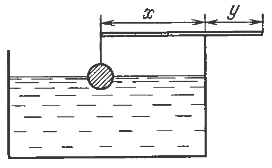
\includegraphics[width=4cm]{fbs03.png}}

\taskpic{На пустую катушку магнитофона, делающую одинаковое количество
  оборотов в единицу времени, перематывается магнитная лента. После
  перемотки конечный радиус $r_{\mbox{\textit{к}}}$ намотки оказался в
  семь раз больше начального радиуса $r_{\mbox{\textit{н}}}$. Время
  перемотки ленты равно $t_1$. За какое время $t_2$ на катушку
  перемотается лента такой же длины, но вдвое более
  тонкая?}{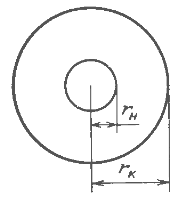
\includegraphics[width=3cm]{fbs04.png}}

\taskpic{Записывая свои воспоминания, барон Мюнхаузен засиделся до
  поздней ночи при свечах. Обе свечи одинаковой длины $l$ он зажег
  одновременно и поставил, как показано на рисунке. Скоро он заметил,
  что тень первой свечи на левой стене неподвижна, а тень второй свечи
  на правой стене укорачивается со скоростью $v$. Через какое время
  барон останется в полной темноте? Считайте, что
  $d_1=d_2=d_3$.}{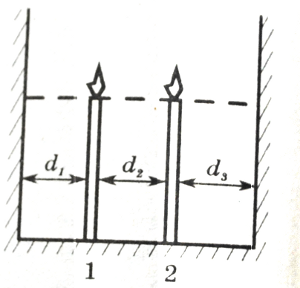
\includegraphics[width=4cm]{fbs05.png}}

\task{Автомобиль проехал половину пути со скоростью $v_1 = 60\mbox{
    км/ч}$. Половину оставшегося времени движения он ехал со скоростью
  $v_2 = 15\mbox{ км/ч}$, а последний участок пути --- со скоростью
  $v_3 = 45\mbox{ км/ч}$. Чему равна средняя скорость автомобиля на
  всем пути?}

\setcounter{notask}{1}

% \begin{center}
 \textsc{Физбой, 9 класс.}
\end{center}
\vspace{0.01cm}
\hrule
\parindent=0mm

\taskpic{Катушка катится без проскальзывания по горизонтальной
  поверхности, причем скорость конца нити (точка~$A$) горизонтальна и
  равна $v$. На катушку опирается шарнирно закрепленная в точке~$B$
  доска. Внутренний и внешний радиусы катушки равны $r$ и $R$
  соответственно. Определите угловую скорость $\omega$ доски в
  зависимости от угла
  $\alpha$.}{
\begin{tikzpicture}
  \draw[interface,thick] (4,0) -- (0.5,0);
  \draw[thick] (2.25,0.75) circle (0.75);
  \draw[thick,dashed] (2.25,0.75) circle (0.35);
  \draw[thick,dashed] (2.25,0.75+0.35) -- ++(0.65,0);
  \draw (2.9,1.1) -- ++(0.5,0);
  \draw[fill=black] (3.4,1.1) circle (0.03) node [above] {$A$};
  \draw[thick,->] (3.4,1.1) -- ++(0.5,0) node [below,midway] {$v$};
  \draw[blue,->] (2.25,0.75) node[above=-2] {\tiny{$r$}} --
  ++(-0.35,0);
  \draw[blue,->] (2.25,0.75)  -- ++(-60:0.75) node[above=2]
  {\tiny{$R$}};
  \draw[very thick] (0.5,0) node [left=-4] {$B$} -- ++(46.5:3.5);
  \draw[blue] (1,0) arc (0:46.5:0.5);
  \draw[blue] (1.15,0.25) node {$\alpha$};
\end{tikzpicture}
}


\task{На тело, движущееся с постоянной скоростью $\vec{v}$, начинает
  действовать некоторая постоянная сила. Спустя промежуток времени
  $\Delta t$ скорость тела уменьшается в два раза. Спустя еще такой же
  интервал времени скорость уменьшается еще в два раза. Определите
  скорость $v_{\mbox{\textit{к}}}$ тела через интервал времени
  $3\Delta t$ с начала действия постоянной силы.}

\taskpic{Для покоящейся системы, изображенной на рисунке, найдите
  ускорения всех грузов сразу после того, как была перерезана
  удерживающая их нижняя нить. Считать, что нити невесомы и
  нерастяжимы, пружины невесомы, масса блока пренебрежимо мала, трение
  в подвесе отсутствует.}{
\begin{tikzpicture}
  \draw[interface,thick] (1,3.5) -- ++(2,0);
  \draw (2,3.5) -- ++(0,-1);
  \draw[very thick] (2,2.5) circle (0.5);
  \draw[thick] (1.5,2.5) -- ++(0,-0.75);
  \draw[thick] (2.5,2.5) -- ++(0,-0.75);
  \draw[thick] (1.25,1.75) rectangle +(0.5,-0.25) node[left=4,midway] {$m_1$};
  \draw[thick] (2.25,1.75) rectangle +(0.5,-0.25) node[right=5,midway] {$m_3$};
  \draw[spring] (1.5,1.5) -- ++(0,-0.5) node [midway,left] {$k$};
  \draw[spring] (2.5,1.5) -- ++(0,-0.5) node [midway,right] {$k$};
  \draw[thick] (1.25,1) rectangle +(0.5,-0.25) node[left=4,midway] {$m_2$};
  \draw[thick] (2.25,1) rectangle +(0.5,-0.25) node[right=5,midway] {$m_4$};
  \draw (2.5,0.75) -- +(0,-0.5);
  \draw[interface,thick] (3,0.25) -- ++(-0.9,0);
\end{tikzpicture}
}

\task{Вблизи поверхности земли свободно падает тело массой $m$. В
  некоторый момент времени в него попадает (и застревает)
  горизонтально летящая тяжелая пуля массой $M$. Определите время
  падения $t$ тела, если известно, что пуля попала в тело на половине
  пути, а время свободного падения тела с той же высоты равно
  $t_0$. Считать, что масса пули много больше массы тела ($M \gg
  m$). Сопротивлением воздуха пренебречь.}

\taskpic{В ведре находится смесь воды со льдом массой $m = 10\mbox{
    кг}$. Ведро внесли в комнату и сразу же начали измерять
  температуру смеси. Получившаяся зависимость температуры от времени
  $T(\tau)$ изображена на графике. Удельная теплоемкость воды равна
  $c_{\mbox{\textit{в}}} = 4{,}2 \mbox{
    кДж}/(\mbox{кг}\cdot\mbox{К})$, удельная теплота плавления льда
  $\lambda = 340 \mbox{ кДж/кг}$. Определите массу
  $m_{\mbox{\textit{л}}}$ льда в ведре, когда его внесли в
  комнату. Теплоемкостью ведра
  пренебречь.}{
\begin{tikzpicture}
  \draw[blue,dashed] (0,2) -- (3,2) -- (3,0);
  \draw[thick,->] (0,0) -- ++(3.5,0);
  \draw[thick,->] (0,0) -- ++(0,3.5) node[right=3,fill=white] {\tiny{$T,
    {}^\circ C$}};
  \draw[very thick,red] (0,0) -- (2.5,0) --
  ($(2.5,0)!1.3!(3,2)$);
  \foreach \x in {20,40,60} {
    \draw (\x/20,0.1) -- ++(0,-0.2) node[below=-3] {\tiny{\x}};
  }
  \foreach \y in {1,2,3} {
    \draw (0.1,\y) -- ++(-0.2,0) node[left=-3] {\tiny{\y}};
  }
  \draw (3.5/2,-0.5) node {\tiny{$\tau$, мин}};
\end{tikzpicture}
}

\task{В схеме, изображенной на рисунке, сопротивления всех
  резисторов одинаковы и равны $R$. Напряжение на клеммах равно
  $U$. Определите силу тока $I$ в подводящих проводах, если их
  сопротивлением можно
  пренебречь.}

\begin{figure}[h]
  \centering
  \begin{circuitikz}[scale=0.8]
    \draw[thick] (4,7) to [generic] (4,4) to [generic] (7,4) to [generic]
    (4,7);
    \draw[thick] (7,4) to [generic] (4,1) to [generic] (4,4);
    \draw[thick] (4,1) to [generic] (1,4) to [generic] (4,7);
    \draw[thick] (1,4) to [generic] (4,4);
    \draw[o-] (1,2) -- (1,4);
    \draw[o-] (2,1) to[out=0,in=-135] (4,4);
    \draw[<->] (1,2) -- (2,1) node [midway,fill=white] {$U$};
    \draw[fill=black] (1,4)  circle (0.1) node [left] {$A$};
    \draw[fill=black] (7,4)  circle (0.1) node [right] {$B$};
    \draw[fill=black] (4,7)  circle (0.1) node [above] {$C$};
    \draw[fill=black] (4,1)  circle (0.1) node [below] {$D$};
    \draw[fill=black] (4,4)  circle (0.1);
  \end{circuitikz}
\end{figure}

\setcounter{notask}{1}

% \begin{center}
 \textsc{Физбой, 10 класс. Полуфинал.}
\end{center}
\vspace{0.01cm}
\hrule
\parindent=0mm

\task{ Тело начинает движение из точки $A$ и движется сначала
  равноускоренно в течение времени $T_0$, затем с тем же по модулю
  ускорением --- равнозамедленно. Через какое время от начала движения
  тело вернется в точку $A$?}

\task{Легкая нерастяжимая нить длиной $2 \unit{м}$ удерживается за
   ее концы так, что они находятся на данной высоте рядом друг с
   другом. На нити висит проволочная скобка в виде перевернутой буквы
   U. Масса скобки равна 1 грамму. Нить выдерживает максимальную
   растягивающую силу $F = 5 \unit{Н}$. ($F \gg mg$). Концы нити
   начинают перемещать в противоположных горизонтальных направлениях с
   одинаковыми скоростями $1 \unit{м/с}$. В какой-то момент нить не
   выдерживает и рвется. На какую максимальную высоту в момент разрыва
   нити взлетит скобка? Сопротивлением воздуха пренебречь.}

 \task{ Две бесконечные пластины толщины $h$ заряжены равномерно по
   объему и сложены вместе. Объемная плотность заряда первой пластины
   $\rho$, а второй $-\rho$. Найдите максимальную напряженность
   электрического поля. }

 \taskpic{ В чёрном ящике находится резистор, имеющий постоянное
   сопротивление и нелинейный элемент, которые могут быть включены как
   последовательно, так и параллельно. Найдите сопротивление
   резистора. Какой нелинейный элемент может находиться внутри чёрного
   ящика? ВАХ для последовательно и параллельно включенных элементов
   представлены на рисунке.}{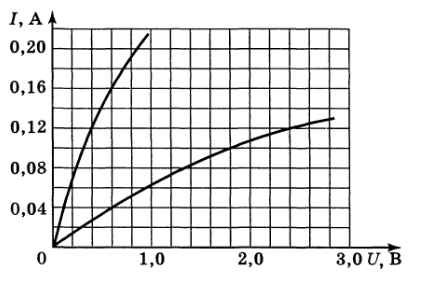
\includegraphics[width=4cm]{fb10_s_1.png}}

 \task{ В чайник с нагревательным элементом мощностью $P$ = 2200 Вт
   налили $V_1 = 1.5 \mbox{ л}$ холодной воды и включили его. когда
   вода закипела, он автоматически отключился. Через $t_1 = 60 \mbox{
     с}$ его снова включили, а еще через $t_2 = 6 \mbox{ с}$ вода
   закипела и чайник выключился. сразу после этого его еще раз
   включили, но сняв крышку. Автоматический выключатель, срабатывающий
   под давлением пара, перестал действовать, и вода из чайника начала
   выкипать. Через $t_3 = 240 \mbox{ с}$ после последнего включения
   измерили объем оставшейся воды. Он оказался равным $V_2 = 1.3
   \mbox{ л}$. Каково значение удельной теплоты парообразования воды
   $L$?  Удельная теплоемкость воды $c = 4200 \mbox{ Дж/(кг*К)}$,
   плотность $\rho = 1000 \mbox{ кг/м}^3$. Теплоемкостью чайника
   пренебречь.}

 \taskpic{ Говорят, что в архиве Снеллиуса нашли рисунок с оптической
   схемой. От времени чернила выцвели, и на бумаге остались видны
   только предмет и его изображение, даваемое тонкой линзой.\\
   1) восстановите построением по имеющимся данным положение линзы.\\
   2) найдите положение фокусов линзы.  \\
   3) можно ли, исходя из рисунка, сказать, какая (собирающая или рассеивающая) была линза?  }{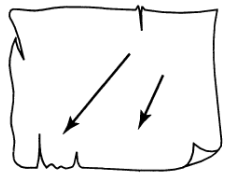
\includegraphics[width=4cm]{fb10_s_6.png}}
\setcounter{notask}{1}


% \begin{center}
 \textsc{Физбой, 10 класс. Финал.}
\end{center}
\vspace{0.01cm}
\hrule
\parindent=0mm

\task{ Над тонкостенным металлическим шаром, радиус которого $R = 5
  \mbox{ см}$, на высоте $h = 10 \mbox{ см}$ находится капельница с
  заряженной жидкостью. Капли жидкости падают из капельницы в
  небольшое отверстие в шаре. Определить максимальный заряд $Q_0$,
  который накопится на шаре, если заряд каждой капли $q = 1.8 \cdot 10^{-11}
  \mbox{ Кл}$. Радиус капель $r = 1 \mbox{ мм}$.}

\task{ Имеется батарейка с эдс $\eps_1$ и внутренним сопротивлением
  $r_1$, а также некоторое количество одинаковых батареек с эдс
  $\eps_2$. Если последовательно с батареей $\eps_1$ подключить
  некоторое количество батареек $\eps_2$ и нагрузку, то сила тока в
  цепи при любом количестве батареек $\eps_2$ будет одинаковой. Если
  же к батарейке $\eps_1$ параллельно подсоединить любое число
  батареек $\eps_2$ и ту же нагрузку, то сила тока через нее останется
  равной прежнему значению. Полярности всех батарей считать
  одинаковыми. Найдите сопротивление нагрузки $R$, а также внутреннее
  сопротивление $r_2$ батареек $\eps_2$.}

\task{ На некоторой планете может быть реализован следующий
  эксперимент. При плоских колебаниях математического маятника длиной
  $L = 3 \mbox{ м}$ максимальная сила натяжения нити отличается от
  минимальной в $k = 4$ раза, если максимальный угол отклонения равен
  значению угла $\alpha$. Такой же угол $\alpha$ с вертикалью образует
  нить маятника, если она вращается с периодом $T = 4 \mbox{ с}$ вокруг
  вертикальной оси, проходящей через точку подвеса. Определите
  ускорение свободого падения на данной палате.  \\
  \textit{Примечание. Частота колебаний математического маятника
    зависит только от длины подвеса и ускорения свободного падения:}
  $\omega = \sqrt{ g/L }$.  }

\task{ Большое число одинаковых плоских монет уложили плоскими
  сторонами вплотную друг к другу, разделив их круглыми кусочками
  бумаги, совпадающими по диаметру с монетами. Получившийся длинный
  цилиндр завернули бумагой в два слоя. Один из торцов этого цилиндра
  касается термостата, имеющего постоянную температуру $Т_1$. Ближайшую к
  термостату монету и сам термостат отделяет кусочек бумаги толщиной
  $h$. Сам цилиндр находится в воздухе, температура которого
  $Т_0$. Теплопроводность монет намного больше, чем теплопроводность
  бумаги. Диаметр монеты $d$, толщина монеты $Н$. Толщина слоя бумаги $h$
  ($h \ll d$). Теплопроводность материала бумаги --- $k$. Со временем
  установилось стационарное распределение температуры. Какое
  количество тепла получает цилиндр из монет от термостата в единицу
  времени?
\\
\textit{  Указание. Тепловой поток $Р$ сквозь тонкий слой вещества, площадь
  которого $S$, а толщина $dx$, равный количеству теплоты, проходящему
  сквозь этот слой в единицу времени, прямо пропорционален разности
  значений температуры его поверхностей $dT$ и обратно пропорционален
  его толщине:
}
  $P = -k S(dT/dx)$, \textit{где $k$ - коэффициент теплопроводности вещества.}
}

\task{ Один конец тонкой гибкой веревки с линейной плотностью $\rho$ тянут
  с постоянной горизонтальной скоростью на высоте $Н$ над шероховатой
  поверхностью. Второй конец веревки свободен. Длина части веревки,
  соприкасающейся с поверхностью равна $l_1$. Найдите длину веревки $l_2$,
  не касающейся поверхности. Коэффициент трения скольжения веревки по
  поверхности равен $k$.}

\task{ Для того, чтобы дорожные знаки были хорошо видны ночью, в
  серебряную краску, которой они покрываются, добавляют стеклянные
  шарики. Каким должен быть коэффициент преломления стекла, чтобы
  такой знак был светоотражающим?}
\setcounter{notask}{1}


% \begin{center}
 \textsc{Физбой, 11 класс. Полуфинал.}
\end{center}
\vspace{0.01cm}
\hrule
\parindent=0mm

\task{Найдите частоту малых колебаний математического маятника
   относительно его нижнего положения равновесия, если непосредственно
   под равновесным положением шарика на расстоянии $h$ от него
   закреплен заряд $Q$. Длина нити $l$, масса шарика $m$, заряд $q$.}

\task{Легкая нерастяжимая нить длиной $2 \mathrm{м}$ удерживается за
   ее концы так, что они находятся на данной высоте рядом друг с
   другом. На нити висит проволочная скобка в виде перевернутой буквы
   U. Масса скобки равна 1 грамму. Нить выдерживает максимальную
   растягивающую силу $F = 5 \mathrm{Н}$. ($F \gg mg$). Концы нити
   начинают перемещать в противоположных горизонтальных направлениях с
   одинаковыми скоростями $1 \mathrm{м/с}$. В какой-то момент нить не
   выдерживает и рвется. На какую максимальную высоту в момент разрыва
   нити взлетит скобка? Сопротивлением воздуха пренебречь.}

\taskpic{Над одним молем идеального газа совершают процесс, показанный на
   рисунке. Найти максимальную температуру газа в течение этого
   процесса (процесс считать квазистатическим)}{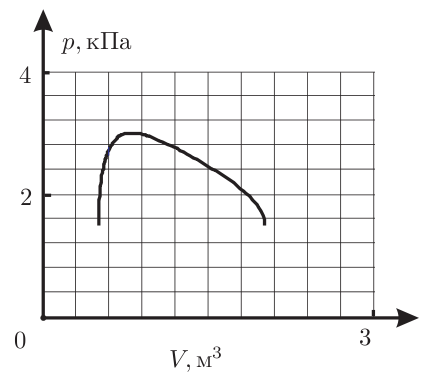
\includegraphics[width=4cm]{fb11_s_3.png}}

\taskpic{C одним молем идеального одноатомного газа провели замкнутый
цикл, изображённый на рисунке, где $1–2$ изотерма, $2–3$ изобара,
$3–4$ политропа, для которой $C = R/2$, и $4–1$ изохора. Минимальная
температура, достигаемая газом в цикле, $T_{min} = 300 \,
К$. Политропическим процессом называется процесс, происходящий с
постоянной теплоёмкостью $C$. Определите КПД цикла
$\eta$.}{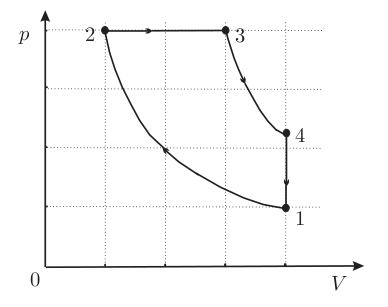
\includegraphics[width=4cm]{fb11_s_4.png}}

\task{В схеме, изображенной на рисунке, имеются четыре диода. Известно, что при любом
   напряжении, подведйнном к выводам схемы, ток через амперметр не течет. ВАХ трех диодов Д1, Д2 и
   Д3 известны (см. график). Постройте ВАХ четвертого диода.
}

\taskpic{В архиве Снеллиуса найден чертеж оптической схемы. От времени чернила выцвели и на чертеже остались видны только
   три точки - фокус линзы F, источник света S, точка L, принадлежащая плоскости тонкой линзы, и часть прямой линии
   а, соединяющий источник света и его изображение S'. Из пояснений к чертежу следует, что точка S' отстоит от
   плоскости линзы на расстояние, большим, чем точка S.
   Возможно ли по этим данным восстановить исходную схему? Если да, то покажите, как это сделать. Чему равно
   фокусное расстояние линзы?
}{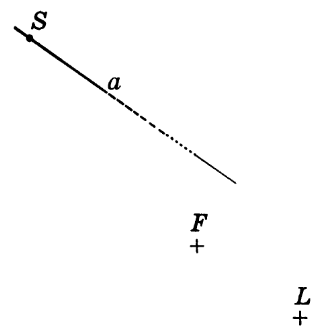
\includegraphics[width=4cm]{fb11_s_6.png}}

\begin{center}
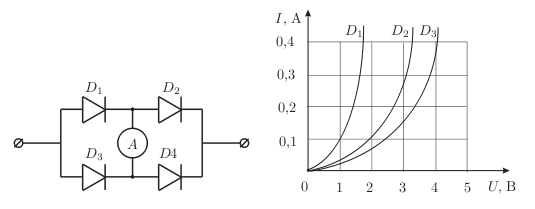
\includegraphics[width=10cm]{fb11_s_5.png}
\end{center}

\setcounter{notask}{1}

% ФИЗБОЙ, СУКА!!!
% 11 КЛАСС

% 1) Электростатика
%    Задача 6.1.14
%    Какой минимальный заряд q нужно закрепить в нижней точне сферической полости радиуса R, чтобы в
%    поле тяжести небольшой шарик массы m и заряда Q находился в верхней точке полости в положении
%    устойчивого равновесия?

%   Замена:
%    Найдите частоту малых колебаний математического маятника относительно его нижнего положения
%    равновесия, если непосредственно под равновесным положением шарика на расстоянии h от него
%    закреплен заряд Q. Длина нити l, масса шарика m, заряд q.

% еще задача 11.7 (Козел)

% 2) Динамика
%    Задача 1.17 (Проволочная скобка)
%    Легкая нерастяжимая нить длиной 2м удерживается за ее концы так, что они находятся на данной высоте рядом друг
%    с другом. На нити висит проволочная скобка в виде перевернутой буквы U. Масса скобки равна 1 грамму. Нить
%    выдерживает максимальную растягивающую силу F = 5Н. (F>>mg). Концы нити начинают перемещать в противоположных
%    горизонтальных направлениях с одинаковыми скоростями 1м/с. В какой-то момент нить не выдерживает и рвется. На
%    какую максимальную высоту в момент разрыва нити взлетит скобка? Сопротивлением воздуха пренебречь.
%    На 10 класс. Если будет совсем уныло - то и на 11ый.

%   Замена:
%    (вроде жесть) 11.84, Козел. На рисунке показана траектория движения лодки, которую
%    оттолкнули от берега рекитак, что в начальнгый момент ее скорость v0 = 1,0 м/с была
%    направлена перпендикулярно берегу. В точке С траектории лодка была через 1 с, в точке D -
%    через 2 с. Определите скорость u течения реки.

% 3) Теплогазы

%    Задача 2.9
%    Над одним молем идеального газа совершают процесс, показанный на рисунке. Найти максимальную температуру газа в
%    течение этого процесса (процесс считать квазистатическим).

%    Экспериментатор Глюк обратил внимание на то, что почти у всех известных ему изопроцессов
%    (изохорического, изобарического, изотермического и адиабатического) график зависимости
%    давления от объема имеет соответствующее название: изохора, ихобара, изотерма и адиабата.
%    У процесса же, в ходе которого не изменяется внутренняя энергия, такого названия нет! Глюк
%    решил восполнить этот пробел и назвал полученную зависимость изоэргой. Далее он решил
%    сравнить ход изоэрги с изотермой и адиабатой для реального одноатомного газа при условиях,
%    близких к нормальным. На рисунке приведены результаты его исследований. Выясните, какому из
%    трех процессов 1-2, 1-3 или 1-4 соответствует "изоэрга", какому - изотерма, а какому -
%    адиабата. Ответ обоснуйте.

%   Замена:
%    Задача 2.7
%    Оцените на какую величину (дельта)х за сутки увеличивается толщина льда, покрывающего водоем, при температуре
%    окружающей среды Т = -20С. В начале похолодания толщина льда была равна 20см. Теплопроводность льда 2.2 Вт/(м*К),
%    его удельная теплота плавления 3.35*10^5 Дж/кг, а плотность 900 кг/см^3.

% 4) Схема

%    Задача 3.7 В схеме, изображенной на рис., имеются четыре диода. Известно, что при любом
%    напряжении, подведйнном к выводам схемы, ток через амперметр не течет. ВАХ трех диодов Д1, Д2 и
%    Д3 известны (см. график). Постройте ВАХ четвертого диода.

%   Замена:

% 5) Оптика

%    11.92, 11.88, 11.54, 11.44!!!!!!!!!!!!




% ---------------------------------------------------------------------------------------------------------------------
% 1) Какой минимальный заряд q нужно закрепить в нижней точне сферической полости радиуса R, чтобы в
%    поле тяжести небольшой шарик массы m и заряда Q находился в верхней точке полости в положении
%    устойчивого равновесия?

% 2) Легкая нерастяжимая нить длиной 2м удерживается за ее концы так, что они находятся на данной высоте рядом друг
%    с другом. На нити висит проволочная скобка в виде перевернутой буквы U. Масса скобки равна 1 грамму. Нить
%    выдерживает максимальную растягивающую силу F = 5Н. (F>>mg). Концы нити начинают перемещать в противоположных
%    горизонтальных направлениях с одинаковыми скоростями 1м/с. В какой-то момент нить не выдерживает и рвется. На
%    какую максимальную высоту в момент разрыва нити взлетит скобка? Сопротивлением воздуха пренебречь.

% 3) Над одним молем идеального газа совершают процесс, показанный на рисунке. Найти максимальную температуру газа в
%    течение этого процесса (процесс считать квазистатическим).

% 4) Оцените на какую величину (дельта)х за сутки увеличивается толщина льда, покрывающего водоем, при температуре
%    окружающей среды Т = -20С. В начале похолодания толщина льда была равна 20см. Теплопроводность льда 2.2 Вт/(м*К),
%    его удельная теплота плавления 3.35*10^5 Дж/кг, а плотность 900 кг/см^3.

% 5) В схеме, изображенной на рис., имеются четыре диода. Известно, что при любом
%    напряжении, подведйнном к выводам схемы, ток через амперметр не течет. ВАХ трех диодов Д1, Д2 и
%    Д3 известны (см. график). Постройте ВАХ четвертого диода.

% 6) В архиве Снеллиуса найден чертеж оптической схемы. От времени чернила выцвели и на чертеже остались видны только
%    три точки - фокус линзы F, источник света S, точка L, принадлежащая плоскости тонкой линзы, и часть прямой линии
%    а, соединяющий источник света и его изображение S'. Из пояснений к чертежу следует, что точка S' отстоит от
%    плоскости линзы на расстояние, большим, чем точка S.
%    Возможно ли по этим данным восстановить исходную схему? Если да, то покажите, как это сделать. Чему равно
%    фокусное расстояние линзы?
% -----------------------------------------------------------------------------------------------------------------------

% Замены:
% 1) Найдите частоту малых колебаний математического маятника относительно его нижнего положения
%    равновесия, если непосредственно под равновесным положением шарика на расстоянии h от него
%    закреплен заряд Q. Длина нити l, масса шарика m, заряд q.

% 2) На рисунке показана траектория движения лодки, которую
%    оттолкнули от берега рекитак, что в начальнгый момент ее скорость v0 = 1,0 м/с была
%    направлена перпендикулярно берегу. В точке С траектории лодка была через 1 с, в точке D -
%    через 2 с. Определите скорость u течения реки.

% 3) Экспериментатор Глюк обратил внимание на то, что почти у всех известных ему изопроцессов
%    (изохорического, изобарического, изотермического и адиабатического) график зависимости
%    давления от объема имеет соответствующее название: изохора, ихобара, изотерма и адиабата.
%    У процесса же, в ходе которого не изменяется внутренняя энергия, такого названия нет! Глюк
%    решил восполнить этот пробел и назвал полученную зависимость изоэргой. Далее он решил
%    сравнить ход изоэрги с изотермой и адиабатой для реального одноатомного газа при условиях,
%    близких к нормальным. На рисунке приведены результаты его исследований. Выясните, какому из
%    трех процессов 1-2, 1-3 или 1-4 соответствует "изоэрга", какому - изотерма, а какому -
%    адиабата. Ответ обоснуйте.

% 4) В чайник с нагревательным элементом мощностью Р = 2200 Вт налили V1 = 1,5л холодной воды и включили
%    его. когда вода закипела, он автоматически отключился. Через t1 = 60с его снова включили, а еще через t2 = 6с
%    вода закипела и чайник выключился. сразу после этого его еще раз включили, но сняв крышку. Автоматический
%    выключатель, срабатывающий под давлением пара, перестал действовать, и вода из чайника начала выкипать. Через
%    t3 = 240с после последнего включения измерили объем оставшейся воды. Он оказался равным V2 = 1,3л. Каково
%    значение удильной теплоты парообразования воды r? Удельная теплоемкость воды с = 4200 Дж/(кг*К), плотность
%    р = 1000 кг/м^3. Теплоемкостью чайника пренебречь.

% 5) Имеется батарейка с ЭДС Е1 и внутренним сопротивлением r1, а также некоторое количество одинаковых батареек
%    с эдс Е2 = Е1/2. Если последовательно с батареей Е1 подключить некоторое количество батареек Е2 и нагрузку, то
%    сила тока в цепи при любом количестве батареек Е2 будет одинаковой. Если же к батарейке Е1 параллельно
%    подсоединить любое число батареек Е2 и ту же нагрузку, то сила тока через нее останется равной прежнему
%    значению. Полярности всех батарей считать одинаковыми. Найдите сопротивление нагрузки R, а также внутреннее
%    сопротивление r2 батареек Е2.

% 6) Говорят, что в архиве Снеллиуса нашли оптическую схему, на которой были изображены линза, предмет - палочка
%    длины l и ее изображение длины l'. От времени чернила выцвели, и остались видны только две точки: вершина
%    палочки S и ее изображение S'. Из текста следовало, что главная оптическая ось проходила через середину палочки
%    перпендикулярно ей. Определите построением положения линзы, главной оптической оси, фокусов линзы, предмета и
%    его изображения и укажите, какая это линза (собирающая или рассеивающая), если l = 5см, l' = 2см, SS' = 15см.


% \begin{center}
 \textsc{Физбой, 11 класс. Финал.}
\end{center}
\vspace{0.01cm}
\parindent=0mm

\taskpic{Определите сопротивление полубесконечной цепочки между точками
  $A$ и $B$, если сопротивление каждого звена равно $R$.}{
\begin{tikzpicture}
  \draw[step=0.5] (0,0) grid (2.9,1);
  \draw[fill=black] (0,0.5) circle (0.05) node[left] {$A$};
  \draw[fill=black] (0.5,0.5) circle (0.05) node[above=7,right=-3]
  {$B$};
  \draw (2.9,0.2) node {$\ldots$};
  \draw (2.9,0.7) node {$\ldots$};
\end{tikzpicture}
}

\taskpic{Человек, стоя на краю высокого обрыва, смотрит на ровное
  плоское дно котлована шириной $L$, заполненного водой глубины
  $h$. Высота обрыва $H$. Размеры котлована удовлетворяют неравенствам
  $L \gg H \gg h$. Показатель преломления воды равен $n$. Как зависит
  от расстояния до обрыва видимая глубина котлована?}{
\begin{tikzpicture}[>=latex]
  \draw[fill=blue!20] (1,1) rectangle ++(3,0.73);
  \draw[thick] (0.5,3) -- ++(0.5,0) -- ++(0,-2) -- ++(3,0) --++(0,2);
  \draw[<->] (3,1) -- (3,1.75) node [midway,right] {$h$};
  \draw[<->] (3,1.75) -- (3,3) node [midway,right] {$H$};
  \draw (1,3) -- ++(-0.1,0.2) -- ++(-0.1,-0.2);
  \draw (0.9,3.2) -- ++(0,0.2);
  \draw (0.9,3.3) -- ++(0.2,0.1);
  \draw (0.9,3.3) -- ++(-0.2,0.1);
  \draw (0.9,3.5) circle (0.1);
  \draw (1,0.75) node {$0$};
  \draw (4,0.75) node {$L$};
\end{tikzpicture}
}

\task{ По диаметру астероида, имеющего форму шара, проходит узкий
  тоннель. С поверхности астероида в тоннель бросили камень, сообщив
  ему скорость, равную первой космической для этого астероида. Через
  какое время камень вернётся назад? Известно, что минимальный период
  обращения космических объектов вокруг астероида равен
  $T_0$. Астероид состоит из однородного вещества, а влияние
  гравитационного поля других небесных тел мало. \\
  \textit{Примечание.} Площадь эллипса $S=\pi ab$, где $a,b$ --- длины
  полуосей эллипса.  }

\task{
  На расстоянии $H$ от бесконечной проводящей плоскости находится
  точечный заряд $q_0$. Найти, на каком расстоянии от проекции заряда
  на плоскость в эту плоскость войдёт силовая линия, вышедшая из
  заряда параллельно плоскости. 
}

\task{
  Один конец тонкой гибкой верёвки с линейной плотностью $\rho$ тянут
  с постоянной горизонтальной скоростью на высоте $H$ над шероховатой
  поверхностью. Второй конец верёвки свободен. Длина части верёвки,
  соприкасающейся с поверхностью, равна $l_1$. Найдите длину верёвки
  $l_2$, не касающейся поверхности. Коэффициент трения скольжения
  верёвки по поверхности равен $k$. 
}

\task{
  Предположим, что создан материал с необычной зависимостью
  коэффициента теплопроводности $k$ от температуры. Пластину из такого
  материала поместили между двумя стенками вплотную к ним. Температуры
  стенок поддерживаются постоянными: $T_1 = 160 K$ и $T_2 = 500 K$
  соответственно. Какой тепловой поток установится между стенками,
  если толщина пластины $d=1 \mbox{ см}$, а её площадь $S= 100 \mbox{
    см}^2$? Найдите температуру в среднем продольном сечении пластины
  ($x=d/2$). \\
\textit{Указание.} Тепловой поток $P$ сквозь тонкий слой вещества,
площадь которого равна $S$, а толщина $dx$, равный количеству теплоты,
проходящему через этот слой в единицу времени, прямо пропорционален
разности значений температуры его поверхностей $dT$ и обратно
пропорционален его толщине: $P = - k S \dfrac{dT}{dx}$, где $k$ ---
коэффициент теплопроводности вещества. 
}

\begin{figure}[h]
  \centering
  \begin{tikzpicture}[>=latex,scale=1.2]
    \draw[help lines,xstep=0.6,ystep=0.35] (0,0) grid (3.4,3.5);
    \draw[thick,->] (0,0) -- (3.6,0) node[above=5,left=-5] {\tiny{$T$, K}};
    \draw[thick,->] (0,0) -- (0,4) node[right=23,below] {\tiny{$k$,Вт/(м$\cdot$К)}};
    \coordinate (a) at (0.8,3);
    \coordinate (b) at (3.2,2.3);
    \coordinate (c) at (1.5,4.3);
    \coordinate (d) at (2.2,0);
    \draw[very thick,red] (a) .. controls (c) and (d) .. (b);
    \draw[blue,dashed] (0.92,0.35*9) -- ++(0,-0.35*9);
    \draw[blue,dashed] (0.6*5,0.35*5.5) -- ++(0,-0.35*5.5) node [below=-1] {\tiny{$T_2$}};
    \draw[blue,->] (0.5,-0.2) node[left=-3] {\tiny{$T_1$}} to
    [out=0,in=215] (0.9,-0.05);
    \draw[thick] (0.6*2,0.15/2) -- ++(0,-0.15) node[below] {\tiny{$200$}};
    \draw[thick] (0.6*4,0.15/2) -- ++(0,-0.15) node[below]
    {\tiny{$400$}};
    \draw[thick] (0.1,0.35*5) -- ++(-0.2,0) node[left=-3] {\tiny{$1$}}; 
    \draw[thick] (0.1,0.35*10) -- ++(-0.2,0) node[left=-3] {\tiny{$2$}};  
  \end{tikzpicture}
\end{figure}


%%% Local Variables: 
%%% mode: latex
%%% TeX-master: "../../../report"
%%% End: 


% \restoregeometry

\parindent=5mm
\subsection{<<Большая Задача>>.}
\label{sec:bz}

<<Большая Задача>> выдаётся командам школьников в начале смены. В
середине смены проводится защита проведённых исследований. В том
случае, если большинство команд справилось с исследованием, выдаётся
вторая <<Большая Задача>>, отчёты по которой защищаются
непосредственно перед окончанием смены. В противном случае, командам
даётся дополнительное время на исследование до конца смены.

\begin{center}
  \textsf{Темы исследований по <<Большой Задаче>>.}
\end{center}

\begin{itemize}
\item \textit{(8-9 класс)} Определить плотность человека.

Командами были предложены следующие методики определения плотности 
человека:
\begin{itemize}
\item измерить ускорение, с которым человек тонет в воде, и, зная 
  массу человека, из этих данных определить плотность;
\item погружаться в воду, прижимая к себе бутылку, частично 
  заполненную водой и частично --- воздухом. Плотность человека 
  рассчитывалась из объема воздуха, необходимого, чтобы человек 
  перестал тонуть;
\item аналогичный метод был предложен и для случая, когда плотность 
  человека меньше плотности воды. В этом случае можно измерить массу 
  песка, которую должен удерживать человек, чтобы начать тонуть;
\item рассчитать плотность человека на основании объема воздуха, 
  который нужно после вдоха выпустить из легких, чтобы начать 
  погружаться в воду;
\item определить плотность на основании измерения доли подводного 
  объема человека в ситуации, когда человек лежит на воде.
\end{itemize}

\item \textit{(8-9 класс)} Исследовать вытекание воды из сифона.

Одна из команд установила, что скорость вытекания воды из сифона 
  пропорциональна квадратному корню из высоты уровня воды над 
  свободным концом трубки.

\com{TODO}

\item \textit{(10-11 класс)} Исследовать силу сопротивления воды. 
\end{itemize}

Приведём отчёт команды, которая по мнению жюри лучше всех
справилась с исследованием. 

\begin{center}
  \large{\textsc{Исследование силы сопротивления воды.}}
\end{center}

\textbf{Состав:} Денис Никитин, Кирилл Михайлов, Антон Терехов,
Дмитрий Жаровов, Александр Косицын (все --- 10 класс). 

\textbf{Цель:} исследовать зависимость силы сопротивления от скорости
тела в воде. 

\begin{center}
  \textbf{Методика.}  
\end{center}

\begin{enumerate}
\item В качестве тела для измерений был выбран шарик для настольного
  тенниса. В него шприцом заливалась вода, что меняло плотность
  шарика.
\item Мячик погружался в воду специально сделанным держателем.
\item В определённый момент мячик отпускали и он поднимался вверх.
\item Вышеописанные действия снимали на видеокамеру с частотой 30
  кадров в секунду. 
\end{enumerate}

\begin{center}
  \textbf{Физическое обоснование.}
\end{center}

\begin{enumerate}
\item Объём шарика мы измерили, обхватив его ниткой. Узнали длину
  окружности и, тем самым, узнали объём.
\item Массу шарика измерили на весах, используя линейку и монеты
  известной массы.
\item Видео, снятое камерой, разбивалось на кадры. Так как около
  ёмкости с водой стояла линейка, то в каждый момент можно было
  определить высоту шарика. Отсюда
  \begin{equation}
    \label{eq:bz_1}
    V = \frac{dh}{dt}, \quad a = \frac{dV}{dt},
  \end{equation}
  где $dt = 1/30$ секунды. Далее, зная ускорение, находим
  \begin{equation}
    \label{eq:bz_2}
    ma = F_a - mg - F_c, \quad F_c = V (g (\rho_{\mbox{ж}} -
    \rho_{\mbox{т}}) - \rho_{\mbox{т}} a). 
  \end{equation}
\end{enumerate}

\begin{center}
  \textbf{Экспериментальные данные. }
\end{center}

Ниже приведены данные, полученные с помощью цифрового фотоаппарата для
трёх различных плотностей груза. 

\begin{table}[ht]
  \centering
  \subfloat[$\rho=910\unit{кг/м}^3$]{
  \begin{tabular}{|c|c|c|}
    \hline
    $v, \unit{м/c}$ & $a,\unit{м/с}^2$ & $F,\unit{Н}$\\
    \hline
    0,06 & 0,9 & 0,002 \\
    \hline
    0,09 & 0,8 & 0,005 \\
    \hline
    0,12 & 0,7 & 0,008 \\
    \hline
    0,14 & 0,6 & 0,011 \\ 
    \hline
    0,16 & 0,4 & 0,017 \\
    \hline
    0,17 & 0,3 & 0,02 \\
    \hline
    0,18 & 0,1 & 0,026 \\
    \hline
    0,19 & 0 & 0,029\\
    \hline
  \end{tabular}}
  \hspace{0.5cm}
  \subfloat[$\rho=740\unit{кг/м}^3$]{
  \begin{tabular}{|c|c|c|}
    \hline
    $v, \unit{м/c}$ & $a,\unit{м/с}^2$ & $F,\unit{Н}$\\
    \hline
    0,16 & 1,2 & 0,056 \\
    \hline
    0,19 & 1,0 & 0,061 \\
    \hline
    0,21 & 0,8 & 0,066 \\
    \hline
    0,23 & 0,7 & 0,068 \\
    \hline
    0,26 & 0,6 & 0,071 \\
    \hline
    0,28 & 0,5 & 0,073 \\ 
    \hline
    0,3 & 0,4 & 0,076 \\
    \hline
  \end{tabular}}
  \hspace{0.5cm}
  \subfloat[$\rho=429\unit{кг/м}^3$]{
  \begin{tabular}{|c|c|c|}
    \hline
    $v, \unit{м/c}$ & $a,\unit{м/с}^2$ & $F,\unit{Н}$\\
    \hline
    0,6 & 4,5 & 0,124 \\
    \hline
    0,71 & 3,3 & 0,141 \\
    \hline
    0,78 & 2,4 & 0,154 \\
    \hline
    0,86 & 1,8 & 0,163 \\
    \hline
    0,9 & 1,3 & 0,170 \\
    \hline
    0,93 & 0,4 & 0,176 \\ 
    \hline
  \end{tabular}}
\end{table}

\begin{figure}[h]
  \centering
  \begin{tikzpicture}
    \begin{axis}[xlabel={$v$, м/с},ylabel={$F$, Н},grid=major,width=10cm,compat=newest,xtick={0,0.04,0.08,0.12,0.16,0.2},xticklabels={0,0.04,0.08,0.12,0.16,0.2}]
      \addplot[thick,color=red,mark=*,error bars/.cd,x dir=both,y dir=both,x
      fixed=0.005,y explicit] coordinates {
        (0.06,0.002) +- (0.01,0.002)
        (0.09,0.005) +- (0.01,0.002)
        (0.12,0.008) +- (0.01,0.002)
        (0.14,0.011) +- (0.01,0.002)
        (0.16,0.017) +- (0.01,0.002)
        (0.17,0.02) +- (0.01,0.002)
        (0.18,0.026) +- (0.01,0.002)
        (0.19,0.029) +- (0.01,0.002)
      };
    \end{axis}
  \end{tikzpicture}
  \caption{График зависимости силы от скорости для $\rho=910 \unit{кг/м}^3$.}
  \label{fig:bz10_1}
\end{figure}

\begin{center}
  \textbf{Теоретическое обоснование. }
\end{center}

Посмотрим на рисунок токов воды во время движения шарика. 

\begin{center}
  \begin{tikzpicture}
    \draw[very thick,fill=gray!30] (3,3) circle (1);
    \begin{scope}[yshift=0.1cm]
      \draw[blue,thick] (6,3) to[out=175,in=0] (3,4.05)
      to[out=180,in=5] (0,3); \draw[blue,thick] (6,3.2)
      to[out=177,in=0] (3,4.15) to[out=180,in=3] (0,3.2);
      \draw[blue,thick] (6,3.4) to[out=180,in=0] (3,4.25)
      to[out=180,in=0] (0,3.4);
    \end{scope}
    \begin{scope}[rotate around={180:(3,3)},yshift=0.1cm]
      \draw[blue,thick] (6,3) to[out=175,in=0] (3,4.05)
      to[out=180,in=5] (0,3); \draw[blue,thick] (6,3.2)
      to[out=177,in=0] (3,4.15) to[out=180,in=3] (0,3.2);
      \draw[blue,thick] (6,3.4) to[out=180,in=0] (3,4.25)
      to[out=180,in=0] (0,3.4);
    \end{scope}
    \draw[fill=black] (2,3) circle (0.05) node[right] {$3$};
    \draw[fill=black] (3,4) circle (0.05) node[below] {$2$};
    \draw[fill=black] (3,2) circle (0.05) node[above] {$1$};
    \draw[fill=black] (3,4.25) circle (0.05) node[above] {$2'$};
    \draw[fill=black] (3,1.75) circle (0.05) node[below] {$1'$};
    \draw[thick,->] (1.5,3) -- (0.75,3) node[left] {$v$};
    \draw[fill=black] (1.5,3) circle (0.05) node[below] {$3'$};
  \end{tikzpicture}
\end{center}


В точках 1 и 2 скорость воды $\approx 0$, а в точках 1' и 2'
находящихся чуть дальше от шарика, $V$. Сила вязкого трения, как
известно, равна $F = \eta S V /d$, следовательно, сила сопротивления
линейно зависит от скорости. 

Заметно, что перед шариком образуется <<водяная подушка>>, область
двигающейся вместе с шариком воды (область между точками 3 и
3'). Поток воды отражается от неё, изменяя импульс шарика: $\vec{F}
\Delta t = m \Delta \vec{V}$. 

\begin{center}
  \begin{tikzpicture}
    \draw[very thick] (4,2) arc (270:165:1.5);

    \draw[blue] (2.85,2.5) ++(-70:0.5cm) arc (-70:-180:0.5cm);

    \draw[thick,->] (1,2.5) -- (2.85,2.5) node[midway,above] {$\vec{V}_1$}; 
    \draw[thick,->] (2.85,2.5) -- ++(-70:1.5cm) node[below] {$\vec{V}_2$};
    \draw[thick,->] (2.85,2.5) -- ++(-125:1cm) node[below] {$d\vec{V}$};
    
    \draw[blue] (2.75,1.75) node {$\alpha$};
    \draw[blue] (2.25,2.15) node {$\alpha$};
  \end{tikzpicture}
\end{center}

Рассмотрим отдельно взятый поток. Его начальная скорость равна
$\vec{V}_1$, конечная~---~$\vec{V}_2$. Так как площадь сечения воды
уменьшается, то $V_2 > V_1$, но незначительно, поэтому мы будем
считать, что $V_1 = V_2$. 

\begin{equation}
  \label{eq:bz_3}
  \vec{V}_1 + d\vec{V} = \vec{V}_2 \quad \Rightarrow \quad dV = V_1 (2 + 2 \cos
  \alpha). 
\end{equation}

При получении $\Delta \vec{V}_0 = \left(\int \Delta \vec{V}  dS \right)
/S$ перпендикулярные скорости шарика проекции взаимоуничтожаются (в
силу симметрии), а параллельные складываются, но все они
пропорциональны $V_1$, поэтому $\Delta V_0 \sim V_1$. 

Запишем закон изменения импульса: 

\begin{equation}
  \label{eq:bz_4}
  F = \frac{m \Delta V_0}{\Delta t} = \frac{S_{\mbox{ш}} V_1 \Delta t
    \rho \Delta V_0}{\Delta t} = S_{\mbox{ш}} \rho V_1 \Delta V_0 \quad
  \Rightarrow \quad F \sim V_1^2.
\end{equation}

Мы видим, что сила сопротивления пропорциональна квадрату скорости
набегающего потока. 

Кроме того, можно заметить, что на больших скоростях сзади шарика
появляется турбулентность, которая изменяет силу сопротивления. 

%%% Local Variables: 
%%% mode: latex
%%% TeX-master: "../../report"
%%% End: 


\com{TODO}

\subsection{<<День Изобретателя>>.}
\label{sec:day_inventor}

День Изобретателя проводится в первое воскресенье смены. Это командное
соревнование, в котором школьники соревнуются в умении сконструировать
действующее устройство, демонстрирующее тот или иной физический
эффект. 

В этом году школьникам 8-9 классов было предложено соорудить
установку, демонстрирующую \textbf{реактивную силу}, а школьникам
10-11 классов~---~установку, выдающую максимально возможную
\textbf{электрическую мощность} (при этом запрещалось использовать
любые готовые источники тока, например, розетки или батарейки). 

\subsection{<<День Экспериментатора>>.}
\label{sec:day_exp}

Во время <<Дня Экспериментатора>> (обычно второе воскресенье смены)
школьники также разбиваются по командам. Всем командам выдаётся
условие двух экспериментальных задач, вместе с необходимым
оборудованием. Далее команды обдумывают методику проведения
эксперимента и рассказывают её членам жюри. После рассказа методики
команды должны продемонстрировать преподавателю ход эксперимента,
провести необходимые измерения и после этого написать отчёт. После
сдачи отчёта команда получает условие новой экспериментальной
задачи. Обычно лучшим командам удаётся решить около 5-6
экспериментальных задач за отведённое время (с 10:00 до 17:00). В
конце дня жюри проверяет отчёты и подводит итоги. Члены победившей
команды получают значки <<Лучший Экспериментатор>>.

Стилистика задач для этого соревнования немного отличается от принятой
на ежедневных занятиях: школьникам даётся минимум оборудования. Это
означает, что методика решения задачи может быть довольно
нестандартной. Например, объект эксперимента может выступать как
измерительный прибор (см., например, задачу №1 в 11 классе). Возможна
и обратная ситуация: измерительный прибор может играть нестандартную
роль (например, с помощью омметра в задаче №7 11 класса
предполагалось заряжать конденсаторы). 

В этом году 8, 9, 10 и 11 класс были поделены на 2, 3, 4 и 4 команды
соответственно. 

\begin{center}
  \textsf{Список экспериментальных задач.}
\end{center}

\begin{itemize}
\item \textbf{8 класс}
  \begin{enumerate}
  \item Измерить толщину бумаги.\\
    \textit{Оборудование:} бумага, линейка.
  \item Измерить силу отрыва магнита от куска железа. \\
    \textit{Оборудование:} магнит, монетки, резинка.
  \item Измерить плотность камня и бруска.\\
    \textit{Оборудование:} камень, брусок, вода, линейка, нитки.
  \item Измерить скорость ветра.\\
    \textit{Оборудование:} бумага, скотч, линейка.
  \item Измерить скорость вытекания воды из крана.\\
    \textit{Оборудование:} секундомер, бумага, пакет, линейка, камни.
  \end{enumerate}
\item \textbf{9 класс}
  \begin{enumerate}
  \item Измерить высоту дерева. \\
    \textit{Оборудование:} линейка.
  \item Измерить плотность неизвестной жидкости.\\
    \textit{Оборудование:} вода, линейка, нитки, камни, кружка,
    неизвестная жидкость.
  \item Измерить разрешающую способность глаза. \\
    \textit{Оборудование:} линейка.
  \item Измерить толщину карандашной линии. \\
    \textit{Оборудование:} карандаш, бумага, линейка.
  \item Измерить плотность масла. \\
    \textit{Оборудование:} вода, масло, 2 трубки, линейка.
  \item Измерить амплитуду дрожания рук экспериментатора. \\
    \textit{Оборудование:} лазерная указка, бумага, карандаш, линейка.
  \end{enumerate}
\item \textbf{10 класс}
  \begin{enumerate}
  \item Измерить отношение радиуса острия булавки к радиусу её
    головки. \\
    \textit{Оборудование:} булавка, фольга, миллиметровка.
  \item Измерить силу отрыва скотча от мотка. \\
    \textit{Оборудование:} скотч, резинка, линейка, монетки.
  \item Измерить длину футбольного поля. \\
    \textit{Оборудование:} линейка.
  \item Измерить угловой размер Солнца. \\
    \textit{Оборудование:} линейка. 
  \end{enumerate}
\item \textbf{11 класс}
  \begin{enumerate}
  \item Измерить коэффициент трения верёвки о трубу. \\
    \textit{Оборудование:} верёвка.
  \item Измерить расстояние между витками в лампочке.\\
    \textit{Оборудование:} батарейка, фольга, провода, игла, линейка,
    бумага, пластилин.
  \item Измерить высоту облаков. \\
    \textit{Оборудование:} линейка.
  \item Измерить отношение теплопроводностей двух металлов. \\
    \textit{Оборудование:} свечка, две проволоки из разных металлов,
    линейка.
  \item Измерить солёность раствора. \\
    \textit{Оборудование:} соль, монетки, линейка, вода, раствор, два
    стакана.
  \item Расшифровать электрический чёрный ящик. \\
    \textit{Оборудование:} чёрный ящик, мультиметр.
  \item Измерить отношение ёмкостей двух конденсаторов. \\
    \textit{Оборудование:} мультиметр. 
  \end{enumerate}
\end{itemize}

В целом, все предложенные задачи были успешно решены
командами. Наиболее активно школьники проявили себя в 9 и 11 классе (в
последнем пришлось выдавать дополнительную задачу, чтобы выявить
победителя). Задачи, предложенные в 10 классе, по-видимому, оказались
довольно сложными с технической точки зрения (так, задачу №1 решила
всего одна команда). 

\com{TODO}

\section{Развлекательная часть.}
\label{sec:fun}

Во второй половине дня в ЛФШ проводятся различные традиционные игры и
состязания. После ужина у школьников обычно свободное время. В это
время обычно проходил факультатив по истории Великой Отечественной
Войны, либо демонстрировались различные художественные фильмы. Кроме
того, после ужина проходили матчи чемпионата по футболу, поскольку
именно в это время суток температура воздуха становилась приемлемой
для игры в футбол.

\end{document}